% !TeX root=../../../main.tex

\chapter{نتایج تجربی}
% دستور زیر باعث عدم‌نمایش شماره صفحه در اولین صفحهٔ این فصل می‌شود.
%\thispagestyle{empty}

\section{پایگاه داده‌های ورودی}
قبل از اینکه وارد روش پیشنهادی شویم به تشریح وردی‌های مسئله و داده‌هایی که مورد استفاده قرار خواهیم داد می‌پردازیم.
داده‌های ورودی برابر ماتریس $D_{m\times n}$ می‌باشد که بعد اول $M$ برابر با ژن‌ها و بعد دوم $N$ برابر سلول‌های نمونه‌برداری شده می‌باشد. در هر خانه $d_{i,j}$ یک بردار داده قرار دارد که حاوی اطلاعات ژن $j$ در سلول $i$ می‌باشد.

\subsection[پایگاه داده مصنوعی]
{پایگاه داده مصنوعی
	\LTRfootnote{Synthetic Dataset}
}

با توجه به این نکته که از درخت فیلوژنی حقیقی\LTRfootnote{Ground-truth Phylogeny Tree} داده‌های حقیقی موجود اطلاعی نداریم، به سراغ ساخت پایگاه‌ داده مصنوعی می‌رویم. با استفاده از این پایگاه داده مصنوعی می‌توانیم در مورد روش‌هایی که در ادامه بیان خواهیم کرد یک معیار ارزیابی نسبتا مناسبی داشته باشیم و تا حدودی از مشکلات روش‌های پیشنهادی آکاه شویم و به تصحیح آن بپردازیم. برای ساخت پایگاه داده مصنوعی که همان ماتریس ورودی $D_{m\times n}$ می‌باشد، از دو روش مختلف با دو فرض مختلف استفاده خواهیم کرد که در ادامه به تشریح هر کدام خواهیم پرداخت.
\\
برای ایجاد پایگاه داده در این حالت ابتدا درختی تصادفی با پارامترهای $\zeta, n$ ایجاد می‌کنیم که $n$ تعداد ژن‌ها (جهش‌ها) بوده و $\zeta$ عددی در بازه $(0, \infty)$ است که یک پارامتر کنترلی است که وظیفه‌اش کنترل کلی تعداد نسل‌های مختلف را از یک جمعیت در درخت فیلوژنی می‌باشد.
حال برای تولید پایگاه داده مصنوعی به ترتیب سه گام زیر باید انجام شود.
\begin{itemize}
	\item ایجاد یک درخت فیلوژنی تصادفی
	\item تبدیل درخت فیلوژنی به ماتریس اطلاعات سلول-ژن ($E$)
	\item اضافه کردن نویز به ماتریس $E$ و تبدیل آن به ماتریس نویزی $D$
\end{itemize}
در ادامه هر بخش به صورت جداگانه به تفضیل شرح داده خواهد شد.

\subsubsection{ساخت درخت تصادفی}
برای ساخت درخت تصادفی از دو روش مختلف استفاده شده است که هرکدام جداگانه توضیح داده شده است.
\vspace{20pt}
\\
\textbf{روش اول: با استفاده از درخت تصادفی دودویی ژنولوژی}\LTRfootnote{Random Binary Genealogical Tree }
\\
در این روش همان‌گونه که از نام آن مشخص است با استفاده از درخت تصادفی دودویی ژنولوژی به ساخت ماتریس داده ورودی مسله می‌پردازیم که برای ساخت این دادگان از فرض‌های که در ادامه آمده است استفاده خواهیم کرد. 

در مرحله اول که ساخت درخت است به این صورت عمل میکنیم که به تعداد $n$ گونه (سلول) در نظر می‌گیریم. سپس به ترتیب مراحل زیر را انجام می‌دهیم تا به درخت تصادفی مورد نظر برسیم.
\begin{itemize}
	\item به هر کدام از $n$ گونه متمایز در ابتدا وزن $w_i=1$ را اختصاص می‌دهیم که متناسب با احتمال انتخاب هر گونه در مراحل بعدی خواهد بود.
	\item برای هر گونه ‌$i$ تابع جرم احتمال را در ادامه به صورت $F_i=\frac{w_i}{\sum_{i=1}^{n}w_i}$ در نظر میگیریم
	\item با استفاده از $F$ دو گونه متمایز $u, v$ را انتخاب می‌کنیم و به هم متصل می‌کنیم
	\item به جای دو گونه $u, v$ یک گونه جدید $uv$ با وزن $w_{uv}=\frac{w_u+w_v}{\sqrt[4]{\zeta}}$ را قرار می‌دهیم.
	\item تعداد گونه‌ها یک واحد کم شده است. بررسی می‌کنیم اگر تعداد گونه‌های باقی‌مانده از $2$ کمتر باشد درخت تصادفی ساخته شده است و پایان کار است. در غیر این صورت به مرحله اول بازمی‌گردیم.
\end{itemize}
پارامتر $\zeta$ به گونه‌ای کنترل‌کننده میزان ناپایداری در طی نسل‌ها می‌باشد. بطوریکه نمونه‌ای از نتایج مقادیر مختلف آن برای $n=20$ در شکل \ref{fig:dsismn20} آورده شده است. پس از ساخت درخت تصادفی به سراغ مرحله بعد یعنی تبدیل درخت به ماتریس ژن-سلول $E$ می‌رویم.
\begin{figure}[!ht]
	\centering
	\subfloat[$\zeta=0.2$]{
			\centering
			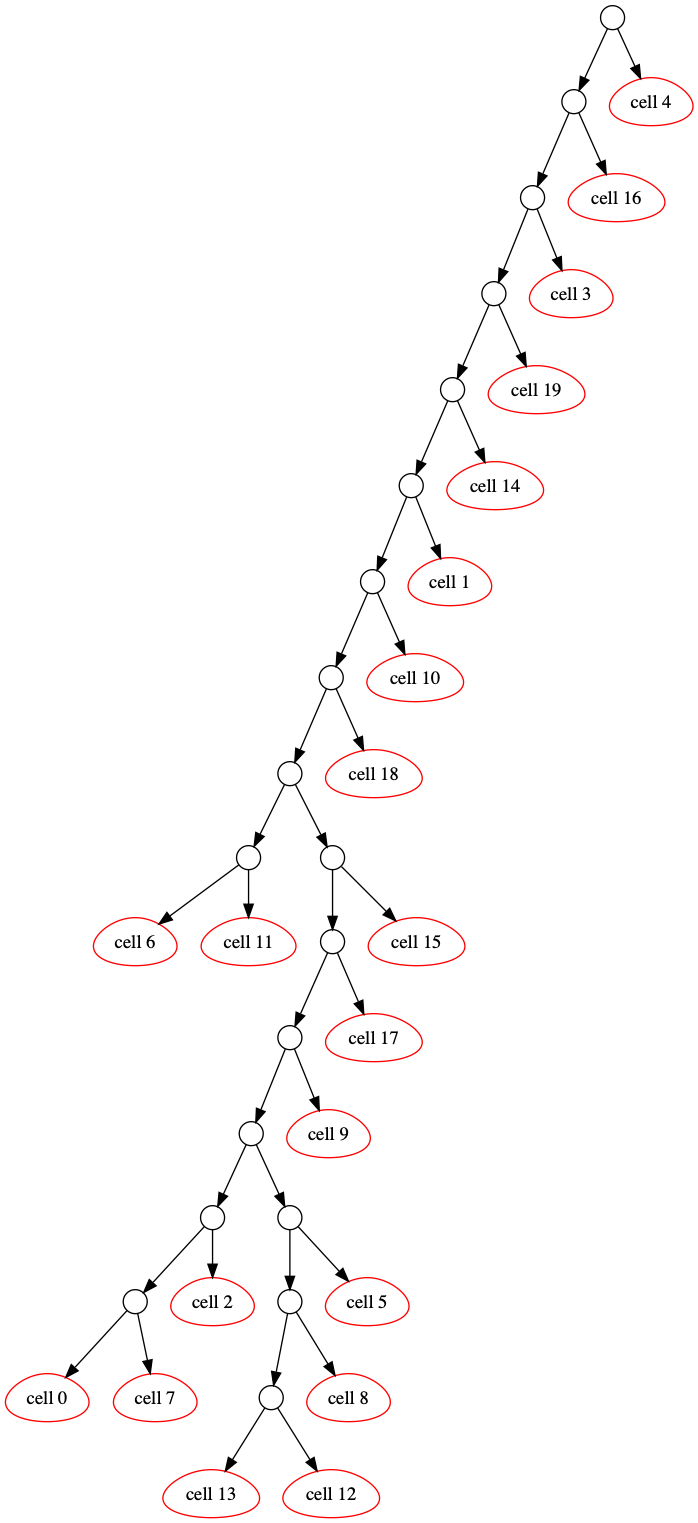
\includegraphics[width=0.48\textwidth, height=0.42\textheight]{img/dataset/s/n20_zeta02}
			\label{fig:dstn20zeta0.2}
	}
	\hfill
	\subfloat[$\zeta=1.0$]{
			\centering
			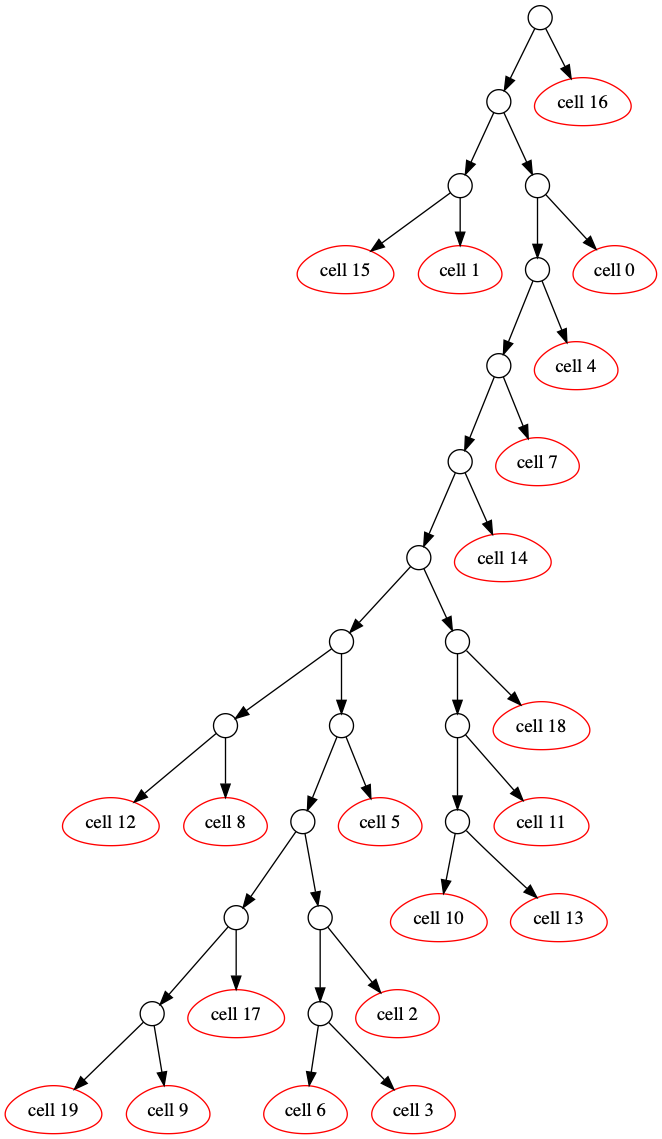
\includegraphics[width=0.48\textwidth, height=0.42\textheight]{img/dataset/s/n20_zeta1}
			\label{fig:dstn20zeta1}
	}
	\hfill
	\vskip\baselineskip
    \subfloat[$\zeta=8$]{
    	\centering
    	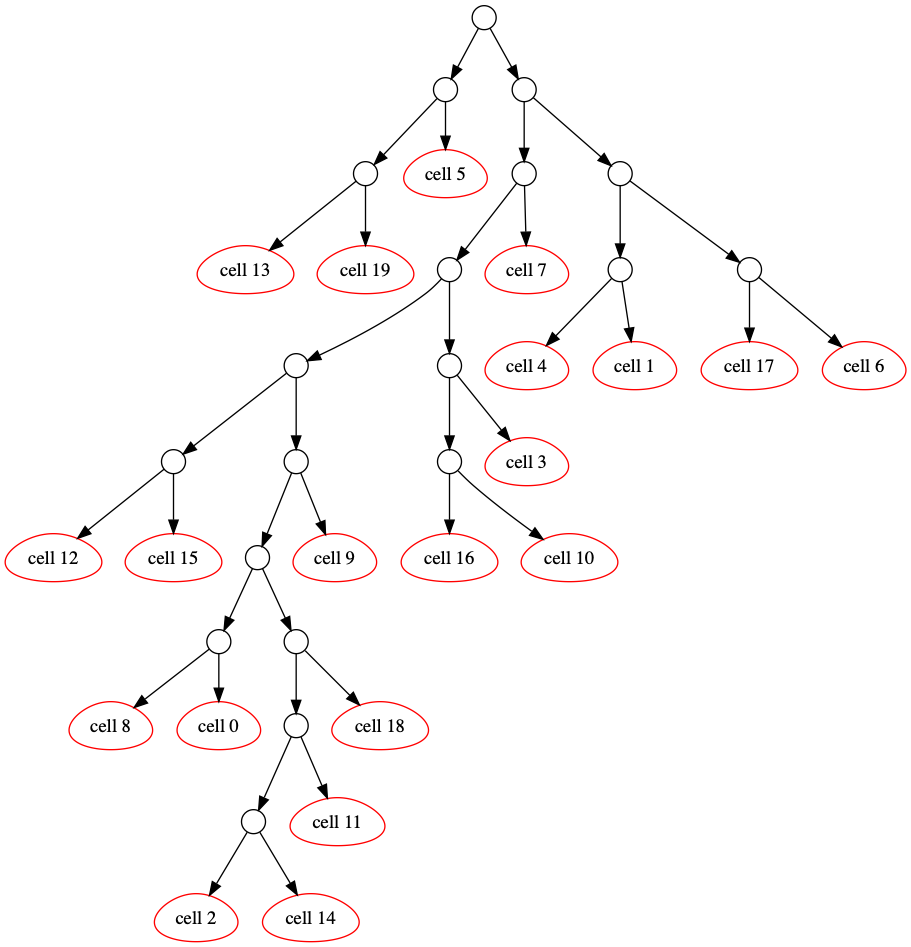
\includegraphics[width=0.38\textwidth, height=0.27\textheight]{img/dataset/s/n20_zeta8}
    	\label{fig:dstn20zeta8}
    }
	\hfill
	\subfloat[$\zeta=100$]{
		\centering
		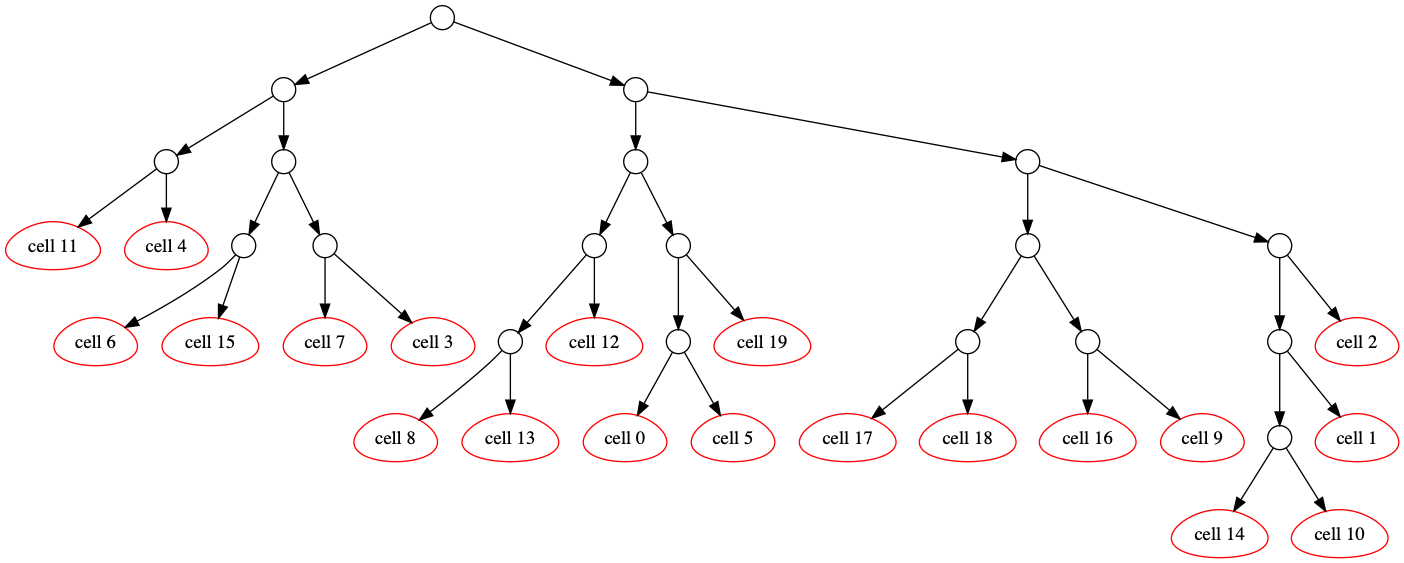
\includegraphics[width=0.58\textwidth, height=0.22\textheight]{img/dataset/s/n20_zeta100}
		\label{fig:dstn20zeta100}
	}
	\caption{درخت فیلوژنی تصادفی تولید شده برای $n=20$ و $\zeta$های مختلف}
	\label{fig:dsismn20}
\end{figure}
\\
در ادامه با توجه به اینکه تعداد دلخواه جهش‌ها چه عددی بوده است یکی از گام‌های زیر را برمی‌داریم.

\begin{itemize}
	\item اگر تعداد جهش‌ها $M>N$ بوده باشد در آن صورت به صورت تصادفی به تعداد دفعات اختلاف یکی از انشعاب‌ها در درخت را به صورت تصادفی انتخاب کرده و آن جهش اضافه شده را تا تمامی نوادگان پیش خواهیم برد.
	\item اگر تعداد جهش‌ها $M<N$ بوده باشد آنگاه مجددا به اندازه تعداد اختلاف انشعاب‌هایی را انتخاب کرده و این بار جهش در آن انشعاب را تا تمامی نوادگان حذف می‌کنیم.  
\end{itemize}
به این ترتیب تمامی سلول‌ها را با تعداد جهش‌های انتخابی خواهیم داشت. در نهایت برای اخرین تغییر در جهش‌ها می‌توان یک گام دیگر برداشت که آن تولید یه عدد تصادفی کوچکتر از $\frac{M}{2}$ است که به آن تعداد می‌توان جهش‌های موجود را از انشعابی برداشت و بر روی انشعابی دیگر قرار داد. با این کار ممکن است تعداد جهش‌ها در انشعاب‌های مختلف تغییر کند و چه بسا به مدل‌های واقعی نزدیکتر شود که البته در این پایان‌نامه از گام آخر صرف‌نظر کرده‌ایم.
\\
حال کار ما با پخش تصادفی جهش‌ها در پایگاه‌داده مجازی پایان یافته است. تا به اینجا ما در فرض خود از هر نمونه جمعیت مختلف یک سلول داشته‌ایم. اما  در بعضی مواقع در پایگاه داده‌های واقعی ممکن است از یک جمعیت بیش از یک نمونه وجود داشته باشد که البته این امر لزوما درست نیست به این دلیل که بعد از افزوده شدن نویز به داده‌ها ممکن است برخی سلول‌ها جهش‌هایشان مشابه هم شود. اما به هرحال اگر چنین چیزی را بخواهیم که داشته باشیم با انتخاب تصادفی برخی سلول‌ها(برگ‌ها) در درخت و کپی کردن آن‌ها می‌توان به چنین مقصودی رسید.
\vspace{20pt}
\\ \textbf{روش دوم: با استفاده از درخت تصادفی جهش‌های ژنی}	\LTRfootnote{Random Mutation History Tree}
\\
این روش نیز تا حدود زیادی مشابه روش قبل است با این تفاوت که در اینجا به جای اینکه درخت تصادفی را با توجه سلول‌ها از پایین به بالا بسازیم، ابتدا یک درخت تصادفی بدون در نظر گرفتن سلول‌ها ایجاد می‌کنیم و سپس به تخصیص جهش‌ها به آن می‌پردازیم و در نهایت برای آخرین مرحله به تعداد دلخواد سلول را به درخت اضافه کرده و درخت را تکمیل می‌کنیم. در گام اول به تعداد $M+1$ نود در نظر میگیریم. مشابه حالت قبل با طی مراحلی بکه در ادامه آمده است به ساختار یک درخت تصادفی می‌رسیم.
\begin{itemize}
	\item به هر کدام از $m$ نود متمایز در ابتدا وزن $w_i=1$ را اختصاص می‌دهیم که متناسب با روند حرکتی تومور به سمت آن جهش‌ها در مراحل بعدی خواهد بود.
	\item برای هر نود ‌$i$ تابع جرم احتمال را در ادامه به صورت $F_i=\frac{w_i}{\sum_{i=1}^{n}w_i}$ بیان می‌شود در نظر می‌گیریم.
	\item با استفاده از $F$ دو نود متمایز $u, v$ را انتخاب می‌کنیم و به هم متصل می‌کنیم
	\item به جای دو گونه $u, v$ یک نود جدید $uv$ با وزن $w_{uv}=\frac{w_u+w_v}{\sqrt[4]{\zeta}}$ را قرار می‌دهیم.
	\item تعداد نود‌ها یک واحد کم شده است. بررسی می‌کنیم اگر تعداد نود‌های باقی‌مانده از $2$ کمتر باشد به مرحله بعد می‌رویم و در غیر این صورت به مرحله اول بازمی‌گردیم.
	\item در این مرحله تمامی برگ‌های درخت ساخته شده را حذف می‌کنیم و تنه باقی‌مانده را به عنوان درخت تصادفی جهش‌ها در نظر می‌گیریم.
\end{itemize}

پس از به پایان رسیدن مراحلی که بیان شد درخت تصادفی آماده است و حال نوبت به تخصیص دادن خود ژن‌ها به هرکدام از این نودهای درخت است. برای این منظور به هرکدام از $M$ نود یک ژن را به صورت تصادفی تخصیص می‌دهیم. پس از آن برای نهایی سازی درخت جهش‌ها از پارامتر دلخواه 	$A = \lfloor\gamma*(M-1)\rfloor$ استفاده می‌کنیم که $\gamma$ عددی بین $(0,1)$ است و $A$ تعداد یال‌هایی است که در درخت باید برداشته شود و دو نود آن با یکدیگر ادغام شود. این کار باعث می‌شود تا در درخت جهش‌ها در برخی نودها به جای یک جهش چند جهش داشته باشیم که بتواند به مدل داده‌های واقعی نزدیکتر باشد.
\\
پس از تکمیل درخت جهش‌ها نوبت قرار دادن نمونه‌هایی بر روی آن است. به همین منظور با فرض اینکه $N\ge M$ است. به تعداد $M$ تا از سلول‌ها را به هر کدام از نودهای درخت جهش به عنوان برگ‌های جدید اضافه می‌کنیم و برای $N-m$ سلول باقی مانده همین کار را این‌بار به صورت تصادفی انجام می‌دهیم. در نهایت درخت تصادفی جهش‌ها ساخته شده است که نمونه‌ای از آن را در شکل \ref{fig:mtn30m20z1g0.15} قابل مشاهده است.
\begin{figure}
	\centering
	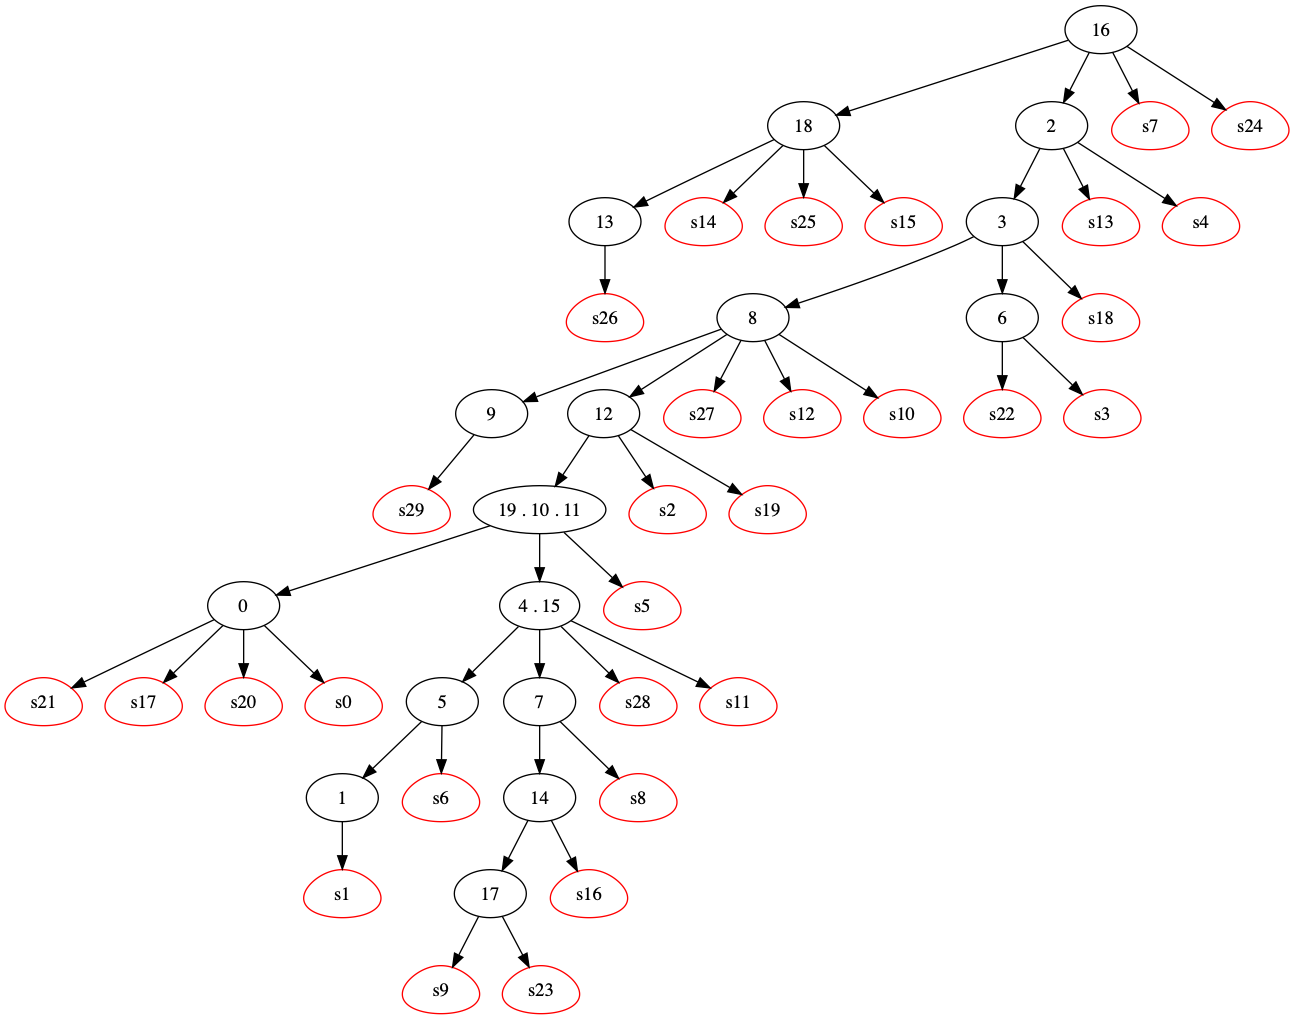
\includegraphics[width=0.75\textwidth]{img/dataset/s/mt_N30_M20_Z1_G0.15_step3.png}
	\caption{درخت جهش تصادفی با پارامتر‌های $N=30, M=20, \zeta=1, \gamma=0.15$}
	\label{fig:mtn30m20z1g0.15}
\end{figure}

\subsubsection{تبدیل درخت به ماتریس ژن-سلول}
با داشتن درخت (تولید شده با هرکدام از روش‌ها تفاوتی ندارد) در ادامه از فرض‌های مختلف در تولید ماتریس $E$ می‌توان استفاده کرد.
\vspace{20pt}
\\
\noindent\textbf{فرض مدل مکان‌های بی‌نهایت}\LTRfootnote{Infinite Site Models}\\
در این حالت فرض می‌کنیم که هر جهش اتفاق افتاده در درخت فیلوژنی در تمامی نسل‌های پس از آن باقی می‌ماند و هیچ‌گاه از بین نمی‌رود. در چنین حالتی درخت حاصل از این روش درختی یکتا بوده که به نام درخت فیلوژنی کامل\LTRfootnote{Perfect Phylogeny Tree} شناخته می‌شود.
\\
در این قسمت باید با استفاده از درخت تصادفی تولید بتوانیم ماتریس جهش‌ها را برای سلول‌های مختلف با فرض مکان‌های بی‌نهایت بدست آوریم. 
در ابتدا ماتریس $E$ را به ابعاد $M\times N$ ایجاد می‌کنیم و برای هر درایه $i,j$ در آن که $i$ شماره جهش و $j$ شماره سلول است به صورت فرمولی که در ادامه آمده است مقداردهی می‌کنیم.
\begin{equation}
	E_{i,j} = 
	\begin{cases} 
		1  \quad &\text{\lr{if}} \quad \text{\lr{mutation }} i \text{\lr{ is an ancestor of cell }} j \\
		0 \quad &\text{\lr{o.w}}
	\end{cases}
\end{equation}
به این ترتیب با فرض مدل مکان‌های بی‌نهایت ماتریس بدون خطا $E$ را داریم که برای تصاویر دو روش درخت مرحله قبل در شکل \ref{fig:E} بدست آمده‌اند.
\begin{figure}[!ht]
	\centering
	\subfloat[ماتریس درخت شکل \ref{fig:dstn20zeta1}]{
		\centering
		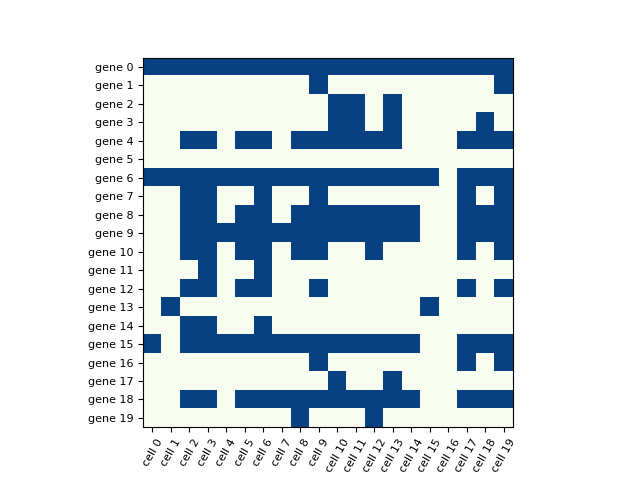
\includegraphics[width=0.48\textwidth]{img/dataset/s/zeta1n20m20}
		\label{fig:Edstn20zeta1}
	}
	\hfill
	\subfloat[ماتریس درخت شکل \ref{fig:mtn30m20z1g0.15}]{
		\centering 
		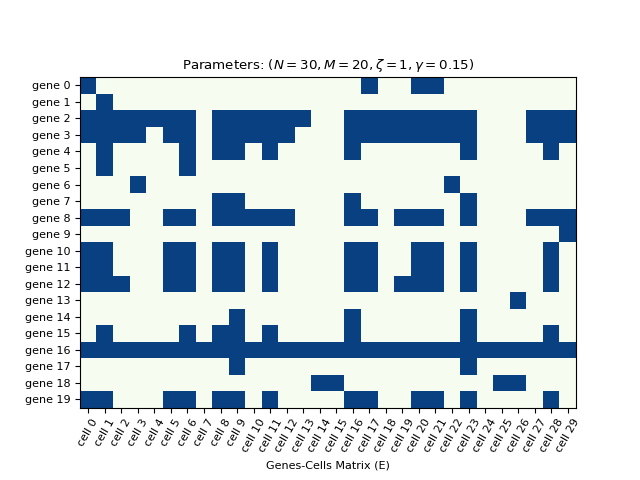
\includegraphics[width=0.49\textwidth]{img/dataset/s/mt_N30_M20_Z1_G0.15_E.png}
		\label{fig:E_mt_N30_M20_Z1_G0.15}
	}
	\caption{ماتریس‌های ژن-سلول ($E$) بدست آمده از درخت‌های تصادفی ساخته شده}
	\label{fig:E}
\end{figure}

\subsubsection{اضافه کردن نویز به ماتریس ژن-جهش}
برای قسمت نهایی آماده سازی پایگاه داده مجازی نیاز است تا به ماتریس $E$ با پارامتر $\Theta=(\alpha, \beta, m_r)$ نویز اضافه کنیم و آن را به ماتریس $D$ تبدیل کنیم که $\alpha=P(D_{ij}=1|E_{ij}=0)$ و $\beta=P(D_{ij}|E_{ij})$ است و همچنین $m_r\in(0,1)$ که نرخ داده‌های از دست رفته را مشخص می‌کند.
\\
برای این منظور به ازای تمامی درایه‌های $0$ ماتریس $E$ هربار یک عدد تصادفی با توزیع یکنواخت بین $[0,1)$ بوجود می‌آوریم و اگر عدد تولید شده کوچکتر از $\alpha$ بود آنگاه ان درایه در ماتریس $D$ را برابر با $1$ قرار می‌دهیم. به همین ترتیب مجددا این بار برای درایه‌های $1$ ماتریس $E$ این‌کار را تکرار می‌کنیم و اگر عدد تصادفی تولید شده کوچکتر از $\beta$ شد، درایه متناظر را در ماتریس $D$ برابر با $0$ قرار می‌دهیم.
\\
پس از اتمام کار نوبت به اضافه کردن داده‌های از دست رفته است. برای این منظور با نرخ $m_r$ بعضی از درایه‌های ماتریس $D$ را برابر با $2$ قرار می‌دهیم که به منزله در دسترس نبودن اطلاعات است. نام ماتریس نهایی را که شامل داده‌های از دست رفته است $D_m$ می‌گزاریم. در ادامه تصاویر اضافه شدن نویز به ماتریس شکل \ref{fig:E_mt_N30_M20_Z1_G0.15} در شکل \ref{fig:D} آمده است.
\begin{figure}[!ht]
	\subfloat[ماتریس نویزی با $\alpha=0.1, \beta=0.08$]{
		\centering
		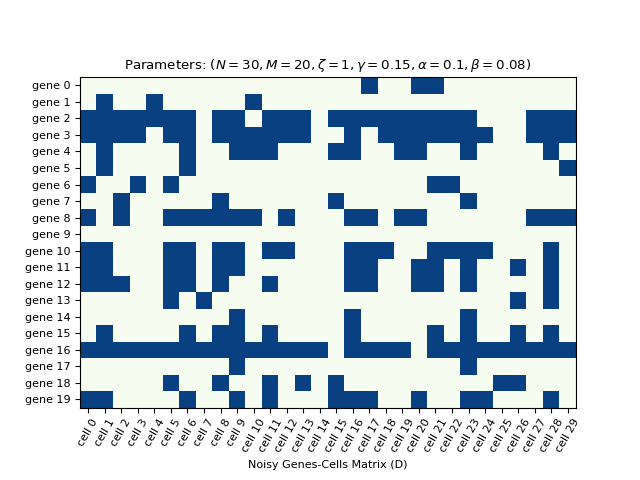
\includegraphics[width=0.5\textwidth]{img/dataset/s/mt_N30_M20_Z1_G0.15_a0.1_b0.08_D.png}
		\label{fig:D_mt_N30_M20_Z1_G0.15}
	}
	\hfill
	\subfloat[نویزی اضافه شده با پارمترهای $\alpha=0.1, \beta=0.08$]{
		\centering 
		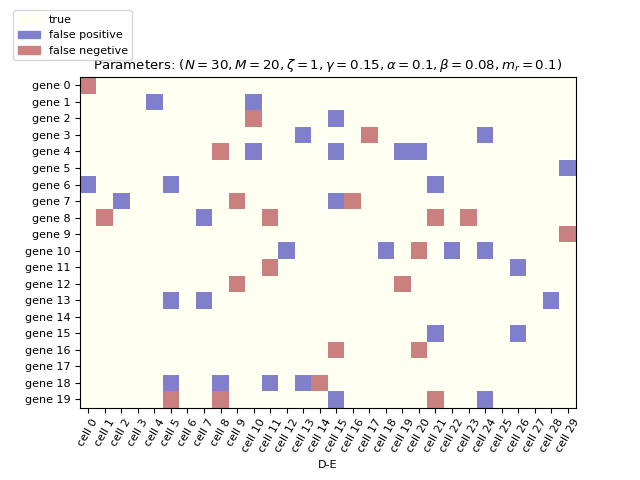
\includegraphics[width=0.5\textwidth]{img/dataset/s/mt_N30_M20_Z1_G0.15_a0.1_b0.08_DmE.png}
		\label{fig:DmN_mt_N30_M20_Z1_G0.15}
	}
	\vskip\baselineskip
	\centering
	\subfloat[ماتریس نویزی به همراه داده‌های از دست رفته با پارامترهای $\alpha=0.1, \beta=0.08, m_r=0.1$]{
		\centering 
		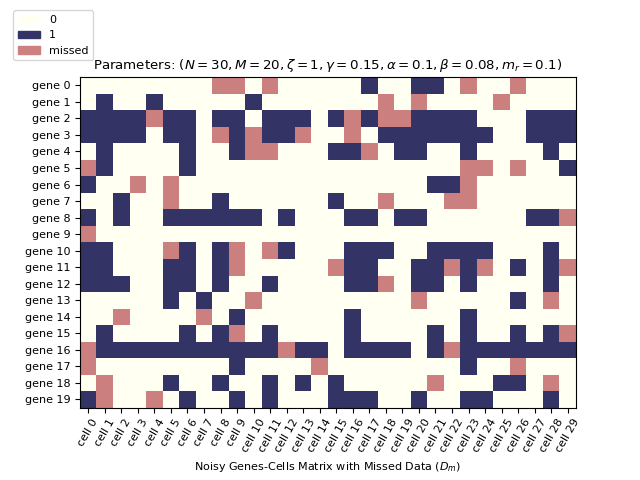
\includegraphics[width=.75\textwidth, height=0.38\textheight]{img/dataset/s/mt_N30_M20_Z1_G0.15_a0.1_b0.08_MR_0.1_Dm.png}
		\label{fig:Dm_mt_N30_M20_Z1_G0.15}
	}
	\caption{ماتریس‌های ژن-سلول همراه با نویز و داده‌های از دست رفته شکل \ref{fig:E_mt_N30_M20_Z1_G0.15} که برای ورودی مسله آماده شده است.}
	\label{fig:D}
\end{figure}


%	\subsubsection[فرض مدل‌های دولو]
%	{فرض مدل‌های دولو
%		\LTRfootnote{Dollo Models}
%	}
%	

\pagebreak
\subsection[پایگاه داده حقیقی]
{پایگاه داده حقیقی
	\LTRfootnote{Real Dataset}
}
به عنوان پایگاه داده حقیقی از پایگاه داده استفاده شده در مقاله \lr{SCITE} به عنوان پایگاه داده حقیقی اصلی استفاده خواهیم کرد که ماتریس داده ورودی آن به صورت شکل  \ref{fig:navin_Dm} می‌باشد.
\begin{figure}[!ht]
	\centering 
	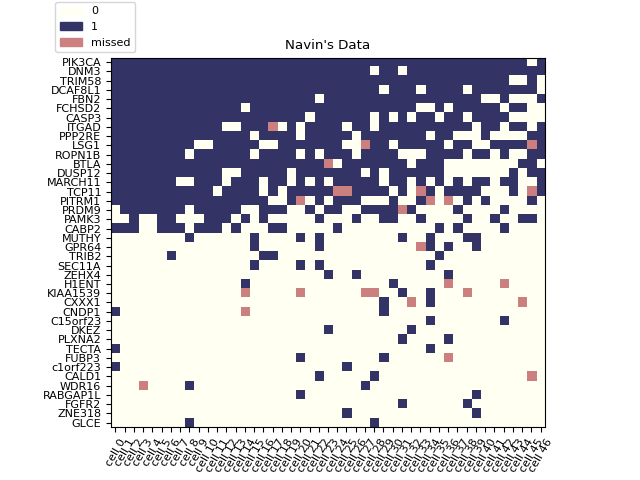
\includegraphics[width=0.67\textwidth]{img/dataset/r/Navin_Dm.png}
	\caption{داده‌های حقیقی \lr{Navin} در مقاله \lr{SCITE}}    
	\label{fig:navin_Dm}
\end{figure}
همچنین پایگاه‌داده حقیقی \lr{Xu} نیز که در مقاله \lr{SCITE} مورد استفاده قرار گرفته است در شکل \ref{fig:Xu_Dm} آمده است.
\begin{figure}[!ht]
	\centering 
	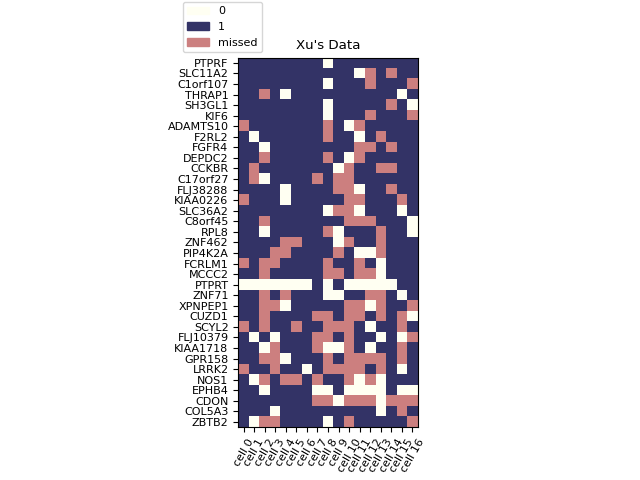
\includegraphics[width=0.625\textwidth]{img/dataset/r/Xu_Dm.png}
	\caption{داده‌های حقیقی \lr{Xu} در مقاله \lr{SCITE}}    
	\label{fig:Xu_Dm}
\end{figure} 

\pagebreak
\section{روش پیشنهادی بدست آوردن درخت فیلوژنی}
پس از تخمین داده‌های از دست رفته، در این بخش به معرفی روش پیشنهادی برای یافتن درخت فیلوژنی می‌پردازیم. در روش‌های گذشته که رویکرد آن در ادامه بیان شده است به موفقیت نرسیدیم و این‌بار در نظر داریم تا با استفاده از یک درخت در ساختار شبکه ژن‌ها بتوانیم به یک درخت فیلوژنی مناسب دست یابیم.  

\begin{itemize}
	\item[-] استفاده از شبکه ژن‌ها
	\begin{itemize}
		\item[\xmark] استفاده از یک  گراف ابتدایی و سپس تغییر و هرس کردنش تا رسیدن به درخت جهش‌ها
		\item[\cmark] استفاده از یک درخت نمونه نابهینه و تغییر اتصالات تا رسیدن به درخت بهینه جهش‌ها
	\end{itemize}
	\item[-] استفاده از شبکه سلول‌ها
	\begin{itemize}
		\item[\xmark] استفاده از یک گراف سلول‌ها و بهینه‌کردن ارتباطات بین آن‌ها و سپس تبدیل آن به درخت فیلوژنی
		%				\item[2.2.] استفاده از یک درخت نمونه نابهینه سلولی و تغییر اتصالات تا رسیدن به درخت بهینه روند تکامل سلولی و تبدیل آن به درخت فیلوژنی
	\end{itemize}
	%		\item[3.]  استفاده از شبکه پیچیده ژن‌-سلول
	%			\begin{itemize}
	%				\item[3.1.] استفاده از یک گراف دو لایه ژن-سلول و بهینه کردن وزن‌ها جهت برش بین دو لایه
	%				\item[3.2.] استفاده از یک گراف پیچیده ژن-سلول و بهینه‌کردن متاپس‌ها
	%			\end{itemize}
\end{itemize}

در رویکرد اول ما از شبکه‌های ژنی استفاده خواهیم نمود. این شبکه‌ها نودهایی معادل با یک ژن متمایز را در نظر می‌گیرند. در گذشته با استفاده از شبکه‌ای کامل با وزن‌های متفاوت که بر حسب اطلاعات ورودی به الگوریتم تعیین می‌شد، متاسفانه به موفقیت خاصی نرسیدیم. همچنین مشابه همین رویکرد را در ساختار شبکه‌های سلولی دنبال کردیم که مجددا پیشرفت قابل ملاحظه‌ای حاصل نشد. به همین جهت این‌بار در این گزارش با تغییری اساسی به دنبال یافتن روشی مناسب برای استنتاج درخت فیلوژنی می‌باشیم.

%
%در رویکرد اول از شبکه ژنی استفاده می‌کنیم. به این ترتیب نودهای ما از جنس ژن‌ها و جهش‌ها بوده و اتصالات بین آن‌ها بواسطه نمونه‌ها (سلول‌ها) که در دسترس هستند رقم خورده و وزن‌دهی می‌شوند. در ادامه نیز با تغییر وزن اتصالات از طریق فرمول‌های مربوطه سعی در یافتن بهترین درختی است که روند به وقوع پیوستن جهش‌های مختلف را در سیر و تحول تومور مربوطه بیان نماید.
%	\\
%	در رویکرد دوم برعکس رویکرد اول نودهای گراف ما نماینده نمونه‌های (سلول‌های) مشاهده شده می‌باشند. به این ترتیب و با توجه به روابطی که برای چنین رویکردی بیان می‌کنیم به تغییر اتصالات و وزن آن‌ها در طی گام‌هایی پشت سرهم می‌پردازیم تا مشخص کنیم که چه نمونه‌هایی بوجود آمده از کدام نمونه‌های دیگر هستند و به عبارتی شجره‌نامه آن‌ها را بیابیم.
%	\\
%	در رویکرد نهایی به استفاده عمیق‌تر از حوزه علوم شبکه برای حل این مسئله می‌پردازیم و با استفاده از دو نوع شبکه مختلف به یافتن پاسخی مناسب برای درخت فیلوژنی می‌پردازیم. در نوع اول که شبکه دولایه است نوع نودهای ما از هر دو نوع ژن و سلول می‌باشد و در طی ارتباطی که هر نوع از نود‌ها با هم دارند معدود اتصالاتی بین این دو لایه وجود خواهد داشت. شبکه دوم نیز مشابه شبکه اول است با این تفاوت که نوع‌های یکسان به یکدیگر اتصال مستقیم ندارند. در ادامه در هر رویکرد به تفضیل در مورد روش استفاده شده در آن توضیح داده خواهد شد.
%	
\subsection{استفاده از شبکه ژن‌ها برای یافتن درخت فیلوژنی}
در این رویکرد با استفاده از شبکه‌ای که نود‌هایی معادل ژن‌ها داشته باشد سعی داریم تا به درخت فیلوژنی بهینه برسیم.

%	\subsubsection{استفاده از یک  شبکه ابتدایی و سپس تغییر و هرس کردنش تا رسیدن به درخت فیلوژنی}
%		احتراما در گزارش بعدی افزوده خواهد شد...
%	در این روش سعی بر این است که از گرافی اولیه که راس‌هایی معادل با ژن‌ها دارد بتوانیم اطلاعاتی استخراج کنیم که توسط آن اطلاعات بتوان ژن‌ها را رتبه‌بندی زمانی کرد. که پس از آن با تغییر گراف بتوان به یک درخت مناسب به عنوان درخت فیلوژنی دست یافت.
%	\\
%	برای این منظور با استفاده از ماتریس داده‌ها $D$ شبکه جهت‌دار کامل $DG$ را با $N$ راس که هر کدام معادل یک ژن در دادگان ورودی است بوجود می‌آوریم که وزن هر اتصال بین $(u,v)$ را به صورت زیر محاسبه کرده و قرار می‌دهیم.
%	\begin{equation}
%		w_{u,v} = 
%	\end{equation}
%	

\subsubsection{استفاده از یک درخت نمونه نابهینه و تغییر اتصالات تا رسیدن به درخت فیلوژنی بهینه}
در این روش قصد داریم تا با شروع از یک درخت نمونه که در ابتدا به صورت تصادفی از اتصال ژن‌ها بوجود آمده است، به بهینه‌ترین درخت ممکن برسیم. این روش به صورت تکرارواره با تغییر اتصالات درخت سعی در بدست آوردن درختی مطلوب‌تر دارد که شرایط و روابط تاثیرگزار در آن به تفضیل شرح داده خواهد شد. در واقع این روش پیشنهادی یک جست‌وجوی حریصانه می‌باشد که طی شرایطی می‌توان انتظار داشت که به پاسخ بهینه دست یافته شود. این روش به نام روش زنجیره مارکو مونت-کارلو\LTRfootnote{Markov Chain Monte Carlo} شناخته می‌شود که در بسیاری از مقالات مرتبط نیز مورد استفاده قرار گرفته شده است.

برای شروع یک درخت تصادفی $T$ را با نودهایی معادل ژن‌های پایگاه داده ورودی در نظر می‌گیریم که در گام اول به صورت تصادفی ساخته شده است. در گام‌های بعدی یک نود $n_1$ را از درخت $T$ به صورت تصادفی انتخاب می‌کنیم. سپس زیردرخت با ریشه این نود را از درخت کم می‌کنیم. حال در درخت باقی‌مانده یک نود دیگر $n_2$ را به صورت تصادفی انتخاب می‌کنیم و آن زیر درخت قبلی با ریشه $n_1$ را به $n_2$ متصل می‌کنیم و درخت جدید را $T_n$ نام‌گزاری می‌کنیم. پس از آن با احتمال،
\begin{equation}
	P=\min\left(1, {Eng(T)\over Eng(T_n)}\right)
	\label{eq:G_Tree_P_Acc}
\end{equation}
درخت جدید بدست آمده $T_n$ را به عنوان نتیجه این گام می‌پذیریم و در غیر این صورت درخت این گام نیز همان درخت سابق $T$ باقی خواهد ماند. در رابطه \ref{eq:G_Tree_P_Acc}، تابع $Eng$ برای یک درخت در واقع انرژی آن درخت را محاسبه ‌می‌کند و ما به دنبال پایدارترین درخت هستیم که کمترین انرژی را داشته باشد. تعریف این تابع برای یک درخت به این صورت است که با توجه به نمونه‌هایی که در دادگان ورودی $D$ قرار دارد و اینکه کدام ژن بالاتر یا پایین‌تر از دیگر ژن‌ها قرار دارد به درخت یک نمره انرژی منصوب می‌کند که به صورت فرمول \ref*{eq:G_Tree_Eng} بیان می‌شود.
\begin{equation}
	Eng(T) = ||E - \hat{E}||
	\label{eq:G_Tree_Eng}
\end{equation}
که در اینجا $\hat{E}$ ماتریس تخمین زده شده روش پیشنهادی با توجه به درخت نهایی بدست آمده خواهد بود. در واقع ماتریس $E$ همان ماتریس صحیح بدون خطا است که جهش‌های مختلف را به ازای سلول‌های مختلف مشخص می‌کند. هنگامی که ما درخت ساخته شده فرضی $T$ را داشته باشیم می‌توانیم در دو گام به $\hat{E}$ برسیم. توجه به این نکته ضروری است که اگر در واقعیت فرض ما که همان مکان بی‌نهایت بود کامل برقرار باشد و $E$ را داشته باشیم، حتما باید بتوانیم به درختی با $Eng(T)=0$ دست یابیم. اما از آنجایی که ما $D$ را به عنوانی از تخمین $E$ داریم بنابرین محاسبه خطای ما نیز تخمینی از خطای واقعی خواهد بود نه خود آن که در اصل به صورت فرمول \ref{eq:Err(T)} می‌شود.
\begin{equation}
	Eng(T) \approx Err(T) = ||D-\hat{E}||
	\label{eq:Err(T)}
\end{equation}

می‌دانیم که هر نود از این درخت $T$ یک مکان برای اتصال سلولی می‌تواند باشد که در این صورت معنی آن اینگونه خواهد بود که سلول ضمیمه شده به آن نود تمام جهش‌های والد خود را داشته است. بنابرین در گام اول نیاز است تا هر مکان از درخت مشخص شود که چه نمونه‌هایی می‌تواند تولید نماید. این اطلاع توسط ماتریس $A$ مشخص می‌شود که به صورت زیر از روی درخت ساخته خواهد شد.
\begin{equation}
	A_{i,j} = 
	\begin{cases}
		1 & \text{اگر $i=j$ یا جهش $i$ والد جهش $j$ باشد}\\
		0 & \text{در غیر این صورت}
	\end{cases}
\end{equation}

حال در گام دوم کافی می‌توانیم با توجه به یک معیار بهترین انتخاب را برای ضمیمه کردن سلول‌ها (نمونه‌های) موجود به درخت داشته باشیم. به همین جهت در ماتریس $D$ که هر ستون آن برابر با نمایش یک سلول است، می‌تواند با هر ستون از ماتریس $A$ مقایسه شود و بهترین ستونی که از $A$ انتخاب شود برابر با جایگاه مناسب ضمیمه شدن نمونه با مقداری خطا به درخت $T$ است. حال با توجه به اینکه فرض مکان‌های بی‌نهایت را داشتیم ماتریس $E$ را به صورت زیر می‌سازیم.
\begin{equation}
	\hat{E}_{i,j} = A_{i, \sigma_j}
\end{equation}
که $\sigma_i$ برابر با بهترین نود (ژن) برای اتصال نمونه  بردار $d_j$ است که بهترین جایگاه به صورت فرمول زیر انتخاب می‌شود.
\begin{equation}
	\begin{aligned}
		\sigma_j = \arg\max_{x\in[1 \to M]}  \sum_{i=1}^M\Big[& \\
		&A_{i,x}D_{i,j}(1-\beta) + (1-A_{i,x})(1-D_{i,j})(1-\alpha) + \\
		&A_{i,x}(1-D_{i,j})\beta + (1-A_{i,x})D_{i,j}\alpha \\
		\Big]& 
	\end{aligned}
\end{equation}
حال با داشتن ماتریس $\hat{E}$ می‌توان خطای درخت را محاسبه نمود و با هدایت \lr{mcmc} طبق فرمول \ref{eq:T_op} به درخت بهینه $T_{op}$ رسید.
\begin{equation}
	T_{op} = \min_{T\in \text{\lr{All possible $T$}}}\Big({||D-\hat{E}_T||}\Big)
	\label{eq:T_op}
\end{equation}



% 
% که تابع $\text{\lr{Parent}}(T,i)$، پدر نود $i$ را در درخت $T$ بازمی‌گرداند و $Pow(i, p)$ به صورت زیر تعریف می‌شود.
% \begin{equation}
% 	Pow(c,p) = \ln\left(\sum_{i=1}^N E(D_{ci}, D_{pi})\right)
% \end{equation}
% این تابع در واقع برای دو ژن که یکی به عنوان پدر دیگری در درخت قرار گرفته است با توجه به نمونه‌های (سلول‌های) در دسترس یک میزان انرژی بدست می‌آورد. هرچه این میزان انرژی کمتر باشد یعنی این نسبت ژنی در درخت پایدارتر و بهینه‌تر است. حال با توجه به اینکه از فرض مدل مکان‌های بی‌نهایت استفاده می‌کنیم، تابع $E$ که در آن مدل‌سازی خطا را نیز لحاظ کرده‌ایم به صورت معادله \ref{eq:G_Tree_E} بیان می‌شود.
% \begin{equation}
% 	E(c, p) = \begin{cases}
% 		(1-\beta)^2e_{1,1} + \alpha^2 e_{0,0} + (1-\beta)\alpha(e_{1,0} +e_{0,1}) & \text{\lr{ if }} c=1,p=1 \\
% 		
% 		(1-\alpha)^2e_{0,0} + \beta^2 e_{1,1} + (1-\alpha)\beta(e_{1,0} +e_{0,1}) & \text{\lr{ if }} c=0,p=0 \\
% 		
% 		(1-\beta)(1-\alpha)e_{1,0} + \alpha\beta e_{0,1} + \alpha(1-\alpha)e_{0,0} + (1-\beta)\beta e_{1,1}) & \text{\lr{ if }} c=1,p=0 \\
% 		
% 		(1-\alpha)(1-\beta)e_{0,1} + \beta\alpha e_{1,0} + (1-\alpha)\alpha e_{0,0} + \beta(1-\beta) e_{1,1}) & \text{\lr{ if }} c=0,p=1 \\
%		\end{cases}
% 	\label{eq:G_Tree_E}
% \end{equation}
% که $\alpha$ و $\beta$ در رابطه \ref{eq:P_alpha_beta} ‌تعریف شده‌اند و $e_{i,j}$ مقدار انرژی است که اگر ژن $i$ به عنوان فرزند $j$ قرار گیرد، با توجه به فرض مدل‌های بی‌نهایت می‌توان به صورت $1\le e_{1,1} \le e_{0,0} < e_{1,0} \ll e_{0,1} $ در نظر گرفت.\\
% همچنین برای سرعت بخشیدن به الگوریتم پیشنهادی می‌توان به جای تغییر یک زیر درخت، دو زیر درخت را با یکدیگر تعویض کرد که در هر گام یکی از این رویکردها به صورت تصادفی انتخاب می‌شود.
%	
%	\subsection{استفاده از گراف سلول‌ها برای یافتن درخت فیلوژنی}
%	احتراما در گزارش بعدی افزوده خواهد شد...
%	
%	\subsection{استفاده از گراف ژن‌-سلول برای یافتن درخت فیلوژنی}
%	احتراما در گزارش بعدی افزوده خواهد شد...

%	\pagebreak
%	\subsection{استفاده از گراف سلول‌ها برای یافتن درخت فیلوژنی}
%	در این رویکرد با استفاده از گراف‌هایی که نود‌های آن برابر با خود سلول‌های نمونه‌برداری شده باشند سعی داریم تا به درخت فیلوژنی بهینه برسیم.
%%	\vspace{20pt}
%%	\subsubsection{استفاده از یک گراف سلول‌ها و بهینه‌کردن ارتباطات بین آن‌ها و سپس تبدیل آن به درخت فیلوژنی}
%	
%	در ابتدا گراف کامل جهت‌دار $DG$ را که هر نود آن معادل یک نمونه سلول است را در نظر می‌گیریم و هر ارتباط $u\rightarrow v$ در این گراف را برابر با احتمال جهش مستقیم سلول $C_u$ به سلول $C_v$ در نظر می‌گیریم که به صورت زیر محاسبه می‌شود.
%	\begin{equation}
%	p(C_u\rightarrow C_v|\Theta) = \prod_i p(C^i_u\rightarrow C^i_v|\Theta)
%	\end{equation}
%	که $C^i_j$ برابر جهش ژن $i$ در سلول $j$ و $\Theta$ برابر با بردار پارامترهای مسئله می‌باشد.
%	\\
%	در ادامه با پیمایش بر روی $DG$ هر ارتباط $u\rightarrow v$ که کم‌احتمال‌تر از مسیری از $u$ به $v$ باشد را حذف می‌کنیم.
%	\\
%	پس از این مرحله برخی از یال‌های گراف حذف خواهد شد.
%	سپس درخت پوشای کمینه را بدست می‌آوریم.
%	\\
%	حال که درخت سلول‌ها را داریم باید آن را به درخت جهش‌ها تبدیل کنیم. این تبدیل به دو صورت می‌تواند انجام شود.
%	\\
%	
%	\noindent\textbf{با فرض مدل مکان‌های بی‌نهایت}\LTRfootnote{\lr{Infinite Site Model}}\\
%	در این فرض جهش‌ها از پدر به فرزندان در درخت به ارث می‌رسد و همیشه در نوادگان باقی می‌ماند. پس در این تبدیل باید جهش‌هایی که برای پدر قرار گرفتن محتمل‌ترند در ارتفاع کمتری قرار گیرند. به همین منظور با استفاده از درخت سلول‌ها یک رتبه‌بندی بین جهش‌ها به صورتی که در ادامه آمده است انجام می‌دهیم
%	\begin{equation}
%		An(G_i \rightarrow G_j) = {C(G_i,G_j) \left(C(G_i, !G_j) - C(G_j, !G_i) \right) \over C(G_i)~C(G_j)} = -An(G_j \rightarrow G_i)
%	\end{equation}
%	در ادامه با استفاده از و کمترین خطایی که در ادامه بوجود می‌آید بتوانیم محتمل‌ترین درخت جهش‌ها را بسازیم
%	
%%	\vspace{20pt}
%%	\subsubsection{استفاده از یک درخت نمونه نابهینه سلولی و تغییر اتصالات تا رسیدن به درخت بهینه روند تکامل سلولی و تبدیل آن به درخت فیلوژنی}
%	
%	
%	\subsection{استفاده از گراف ژن‌-سلول برای یافتن درخت فیلوژنی}
%	

\newpage
\section{نتایج تجربی}
در این بخش به نتایج بدست آمده برای روش پیشنهادی می‌پردازیم و برای هر دو داده مصنوعی و حقیقی نتایج بدست آمده را تحلیل خواهیم نمود.
\subsection{نتایج بر روی پایگاه داده مصنوعی}
همان‌گونه که در بخش دوم توضیح داده شد با توجه به سختی دسترسی به پایگاه داده‌های حقیقی و اینکه در آن‌ها نیز حقیقت داده‌ها ($E$) وجود ندارد تصمیم به ایجاد پایگاه داده‌ای مصنوعی گرفته شد که با کمک آن بتوان ارزیابی مناسبی از روش پیشنهادی و میزان کارایی و مقاومت روش را نسبت به تغییر پارامترها سنجید.

فرض کنید ماتریس ورودی شکل \ref{fig:sy_D1} را در اختیار داریم و میخواهیم بهترین درخت فیلوژنی را برای آن بیابیم.
\begin{figure}[!ht]
	\centering
	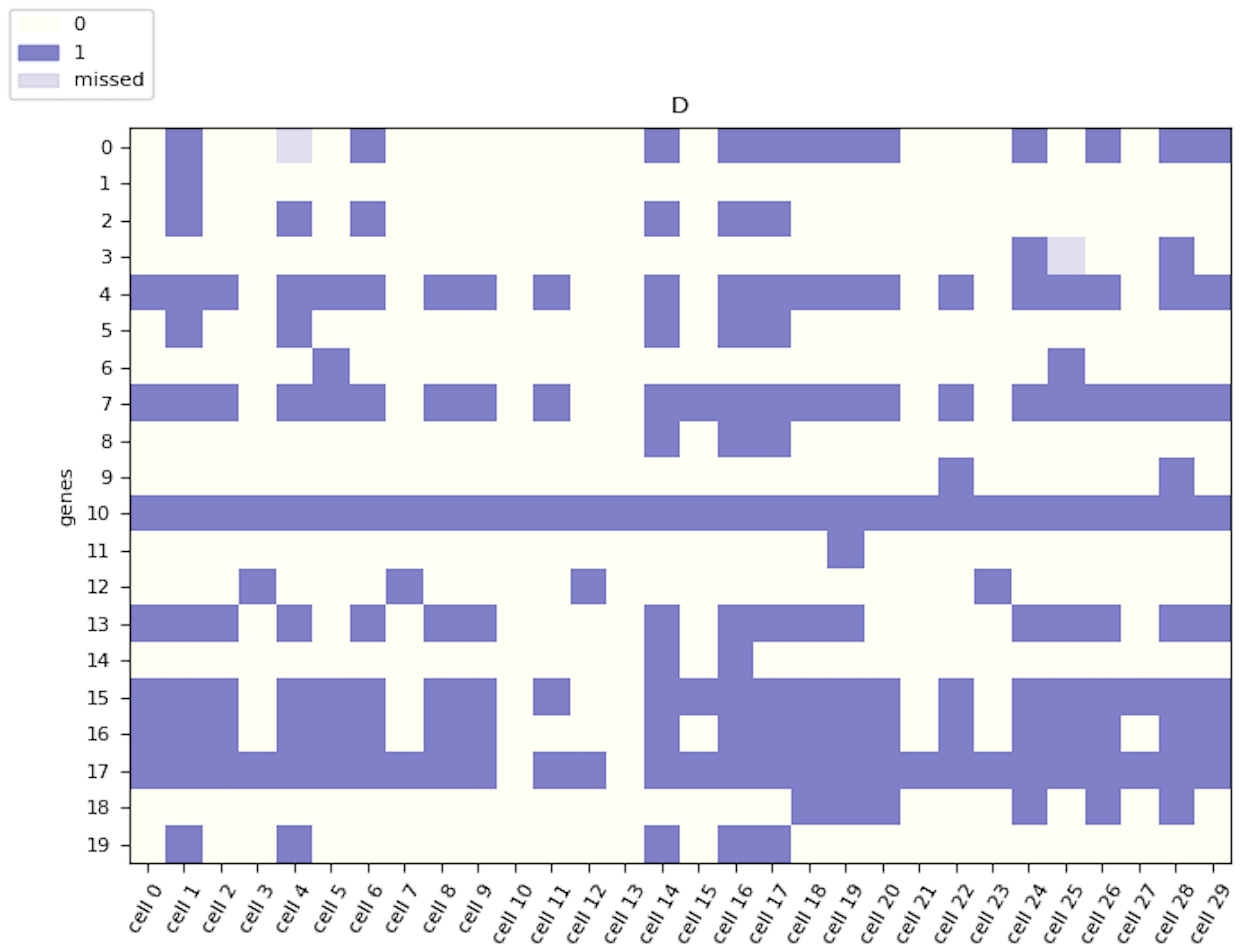
\includegraphics[width=0.7\textwidth]{img/res/D1}
	\caption{نمونه‌ای تصادفی از ماتریس ورودی $D$}
	\label{fig:sy_D1}
\end{figure}

حال یک درخت تصادفی به صورت شکل \ref{fig:sy_initial_T1} می‌سازیم.
\begin{figure}[!ht]
	\centering
	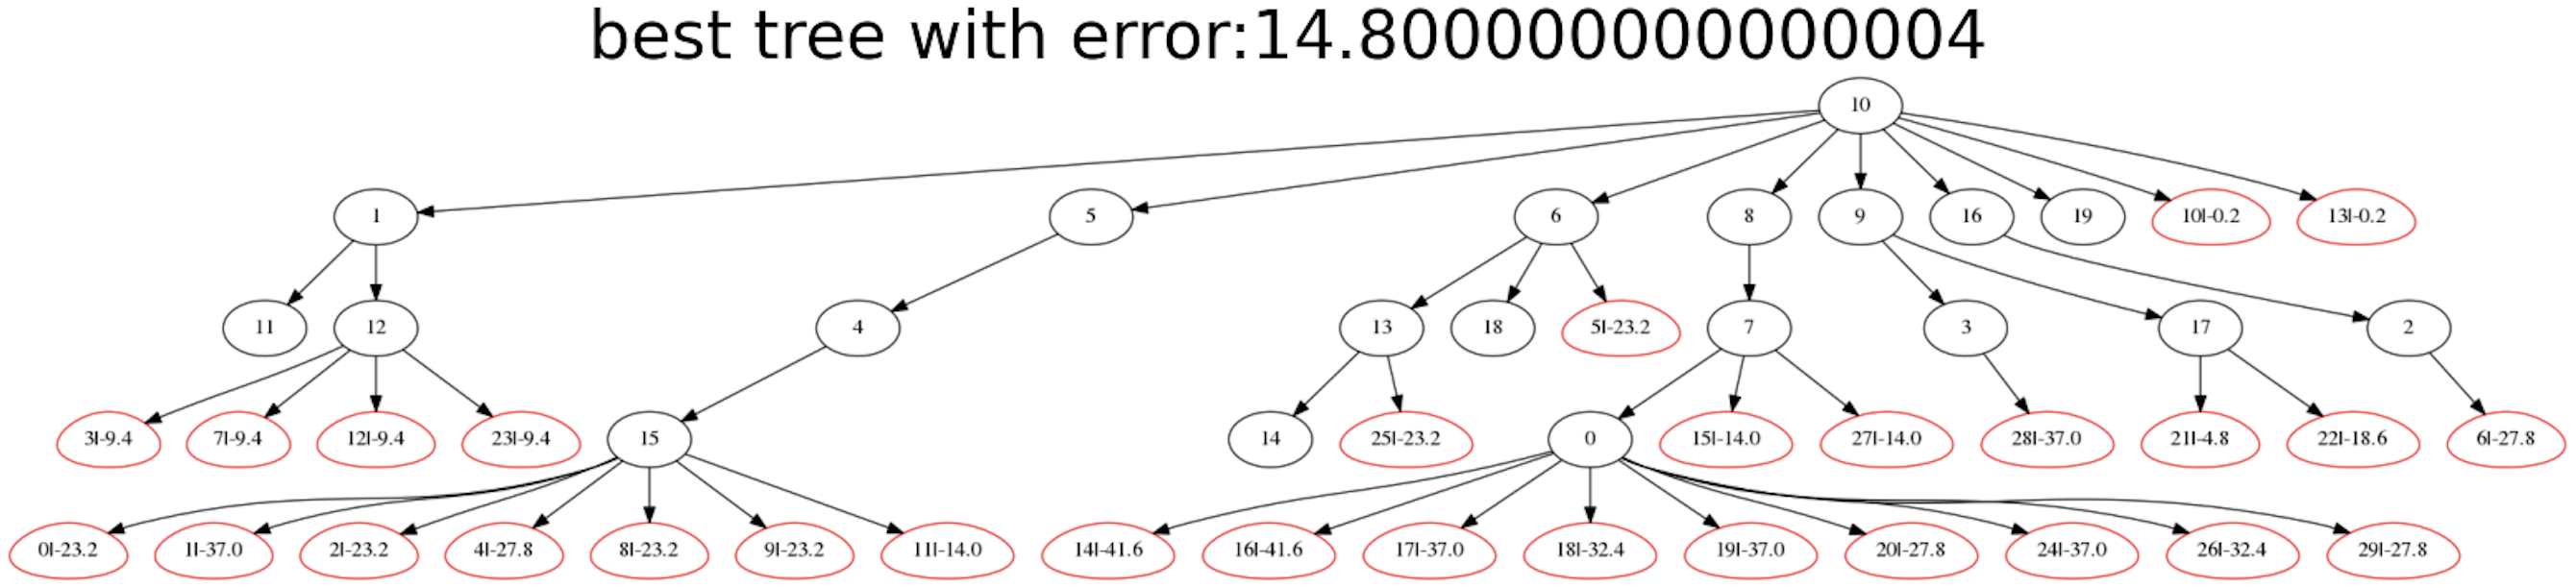
\includegraphics[width=\textwidth]{img/res/initial_T1}
	\caption{‌درخت تصادفی ایجاد شده به عنوان درخت اولیه شکل \ref*{fig:sy_D1}}
	\label{fig:sy_initial_T1}
\end{figure}
در درخت شکل  \ref{fig:sy_initial_T1} نمونه‌ها (سلول‌ها) با رنگ قرمز به درخت متصل شده‌اند که البته این ضمیمه بهترین ضمیمه ممکن است و میزان انرژی (خطای) هر ضمیمه نیز در کادر قرمز رنگ سلول‌ها به صورتی عددی منفی نوشته شده است. 
\\
پس از این مرحله اگر $3000$ گام \lr{MCMC} را اجرا نماییم می‌توانیم نتیجه حاصله را در شکل \ref{fig:sy_benchmark1} مشاهده کنیم. در این شکل دو درخت وجود دارد که درخت سمت راستی درخت حقیقی است که به دنبال آن بودیم و درخت سمت چپ بهترین درخت یافته شده است. همچنین در پایین شکل، ۹ ماتریس مشاهده می‌شود که ماتریس‌ها سمت راست و پایین به نوعی بیان‌کننده میزان خطا بین ۴ ماتریس سمت چپ بالا می‌باشند. در بالای هر ماتریس نام آن نوشته شده است و در نهایت در انتهای تصویر نیز روند کاهش خطا و تلاش‌های \lr{MCMC} در گام‌های مختلف قابل مشاهده است. فقط نکته‌ای که وجود دارد این است که خطای نوشته شده در تصاویر برابر $0.1$ مقیاس نوشته شده است.
\\
همان‌گونه که مشخص است در ماتریس $D$ دو داده از دست رفته وجود دارد که یکی از آن‌ها در حقیقت جهش یافته و دیگر خیر. اگر ما در محاسبات خود این دو داده را در محاسبه خطا در نظر نگیریم و با تغییر ۳ داده دیگر می‌توانیم به ماتریس $\hat{E}$ (در شکل به نام $E$ نوشته شده است) برسیم که معادل بهترین درخت بدست آمده است. که این یعنی ماتریس $D$ ما با ۵ تغییر بدست ما رسیده است. حال اگر حقیقت داده‌ها و درخت اصلی را مشاهده کنیم می‌بینیم که در آنجا نیز ۵ خطا وارد شده است که ۲ تای آن‌ها را درست کشف شده است. بنابرین الگوریتم بدون اطلاع از حقیقت توانسته با حداکثر ۵ خطا به یک درخت فیلوژنی مناسب دست بیابد که در ساختار نیز شباهات بسیار زیادی به حقیقت دارد. بنابرین روش پیشنهادی توانسته درخت فیلوژنی را با صحت 
${20*30 - 5\over 20*30} = 0.991\overline{6}$
بازسازی کند که عددی قابل قبول می‌باشد.

\newpage
\begin{figure}[!ht]
	\centering
	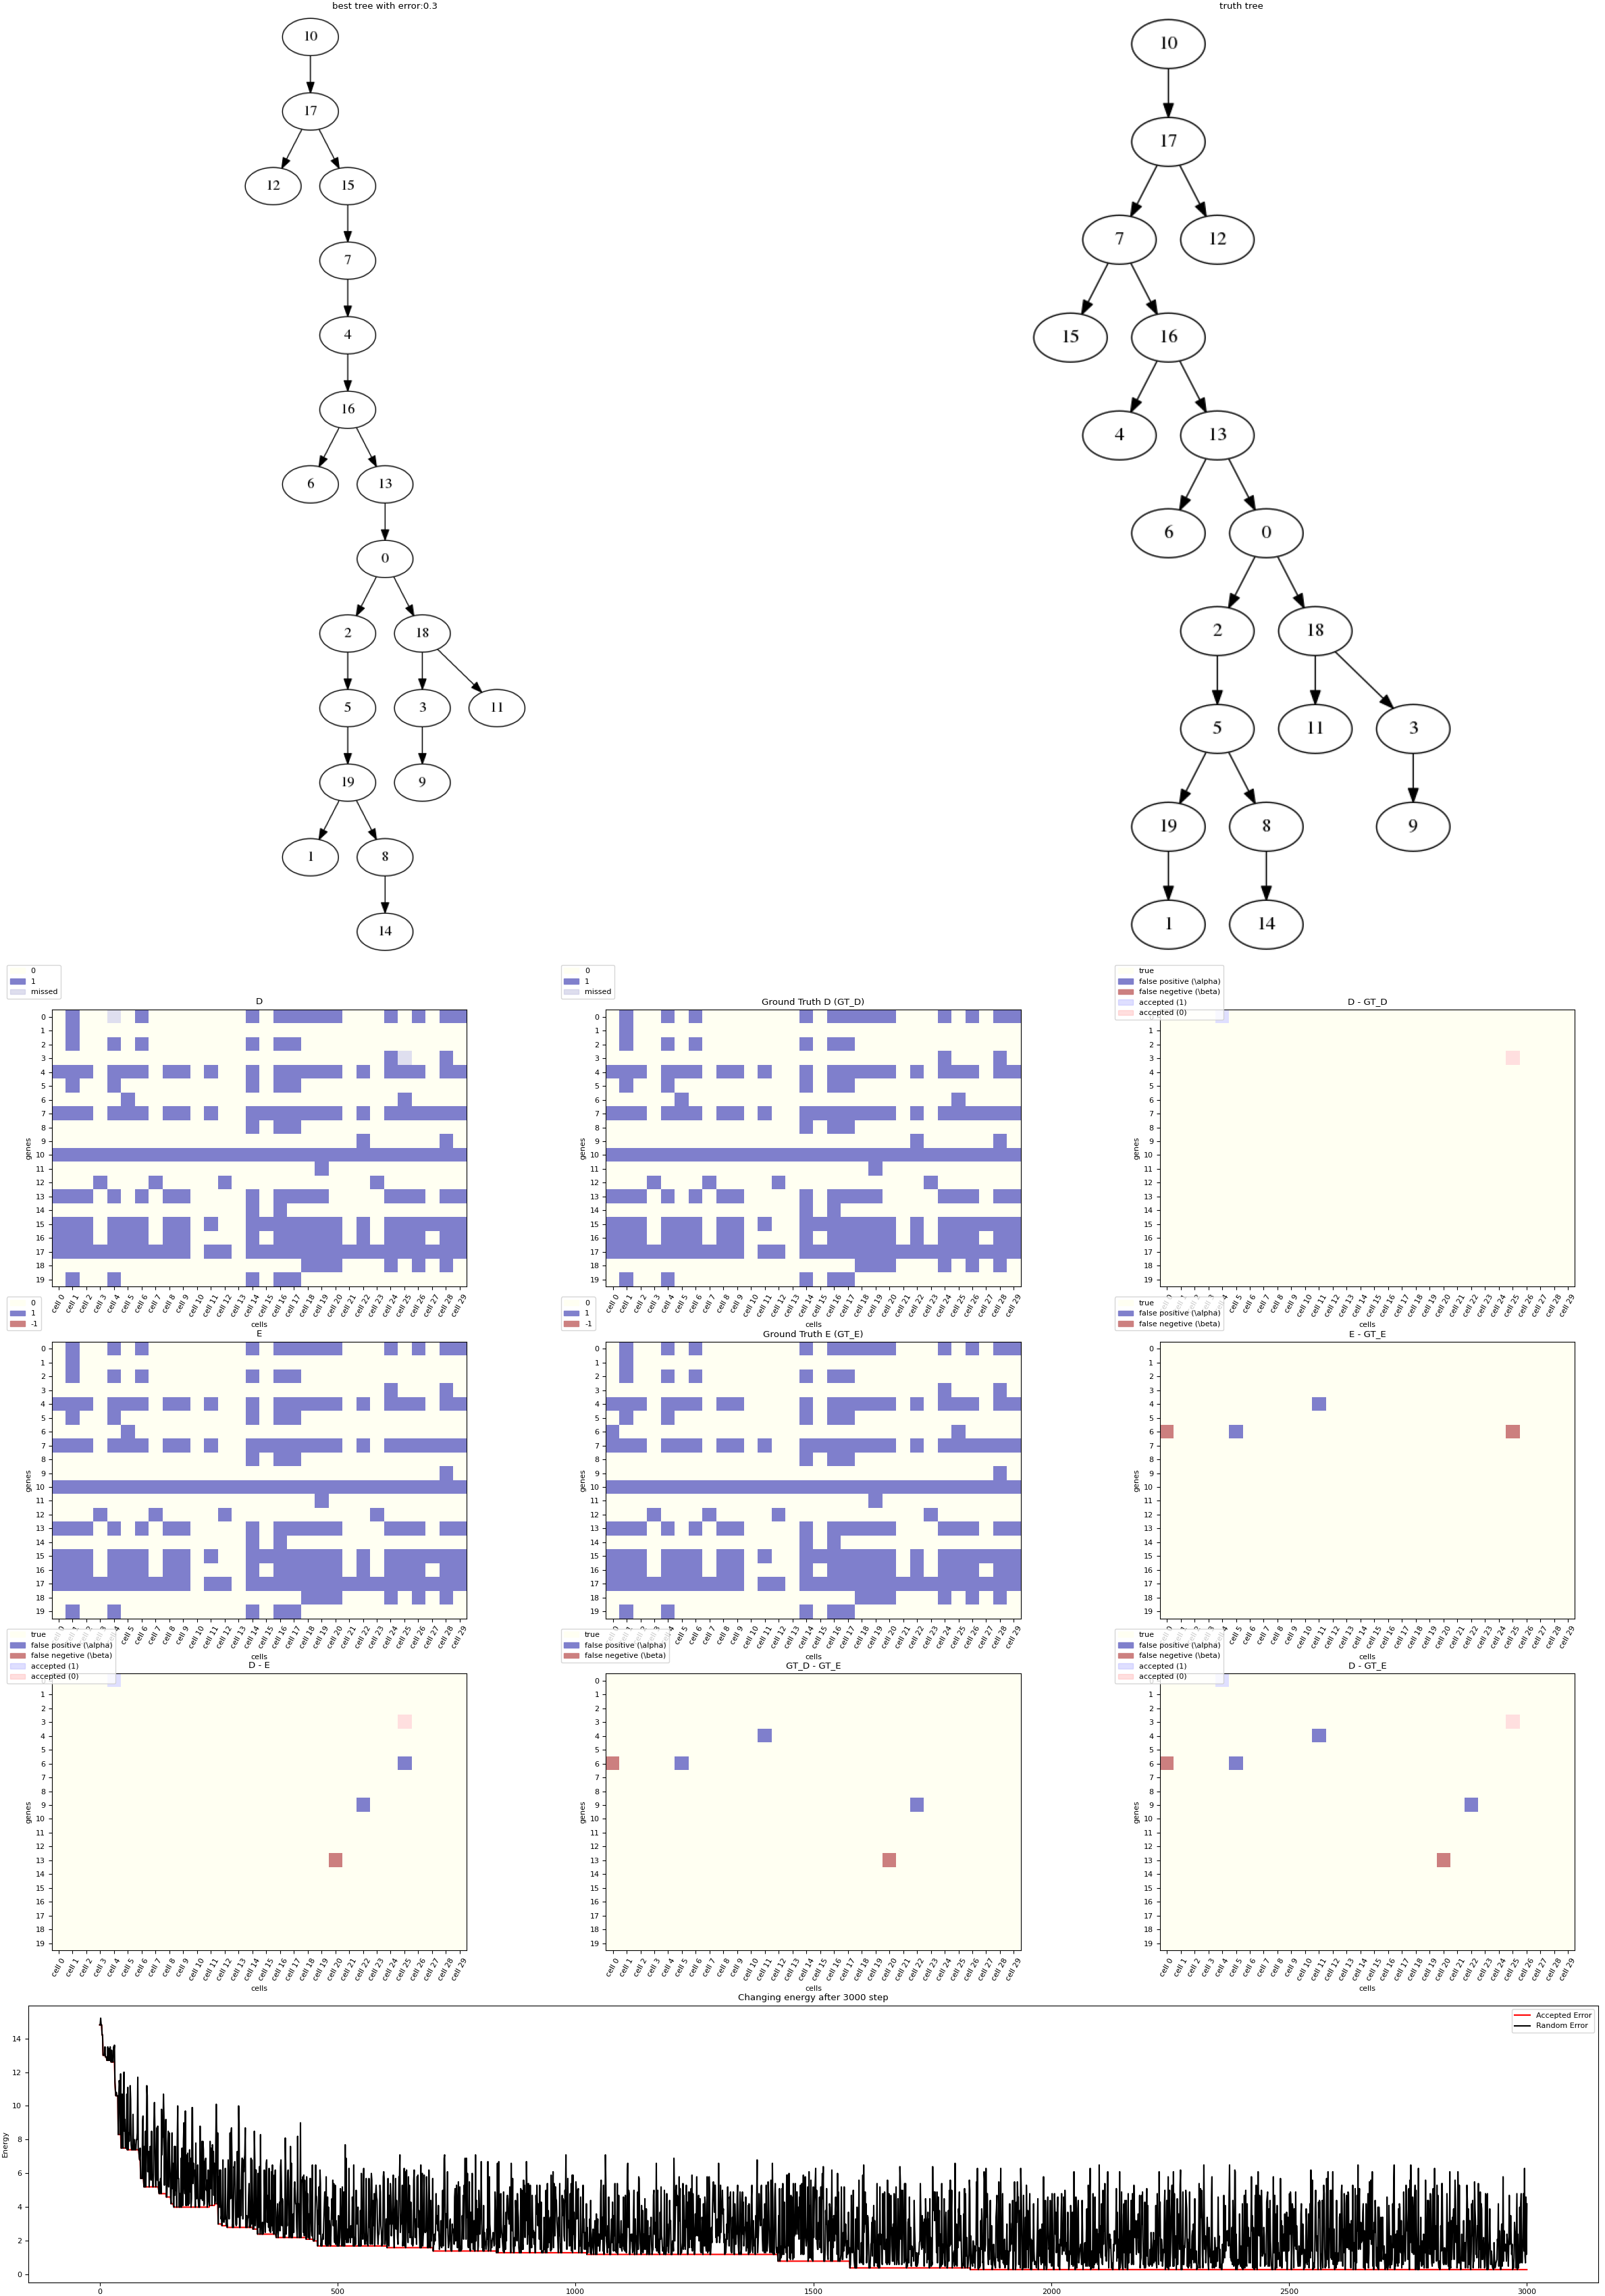
\includegraphics[height=0.9\textheight]{img/res/benchmark1}
	\caption{‌نتیجه اجرای روش پیشنهادی برای ماتریس شکل \ref*{fig:sy_D1}}
	\label{fig:sy_benchmark1}
\end{figure}
\pagebreak
اما برای بررسی مناسب‌تر تعدادی تست را به ازای $M$ و $N$های مختلف اجرا نمودیم که به صورت خلاصه نتایج حاصل از آن در ادامه قابل مشاهده است.
\\
در شکل \ref{fig:sy_n_err} مقدار خطای درخت بهینه یافته شده قابل مشاهده است که نشان می‌دهد هر چه تعداد نمونه‌ها افزایش پیدا میکند و اندازه ماتریس ورودی بزرگ‌تر می‌شود، مقدار خطا نیز افزایش می‌یابد. در این اجرا تعداد جهش‌ها نیز عددی بین تعداد نمونه‌ها و نصف تعداد نمونه‌ها بوده است.
\begin{figure}[!ht]
	\centering
	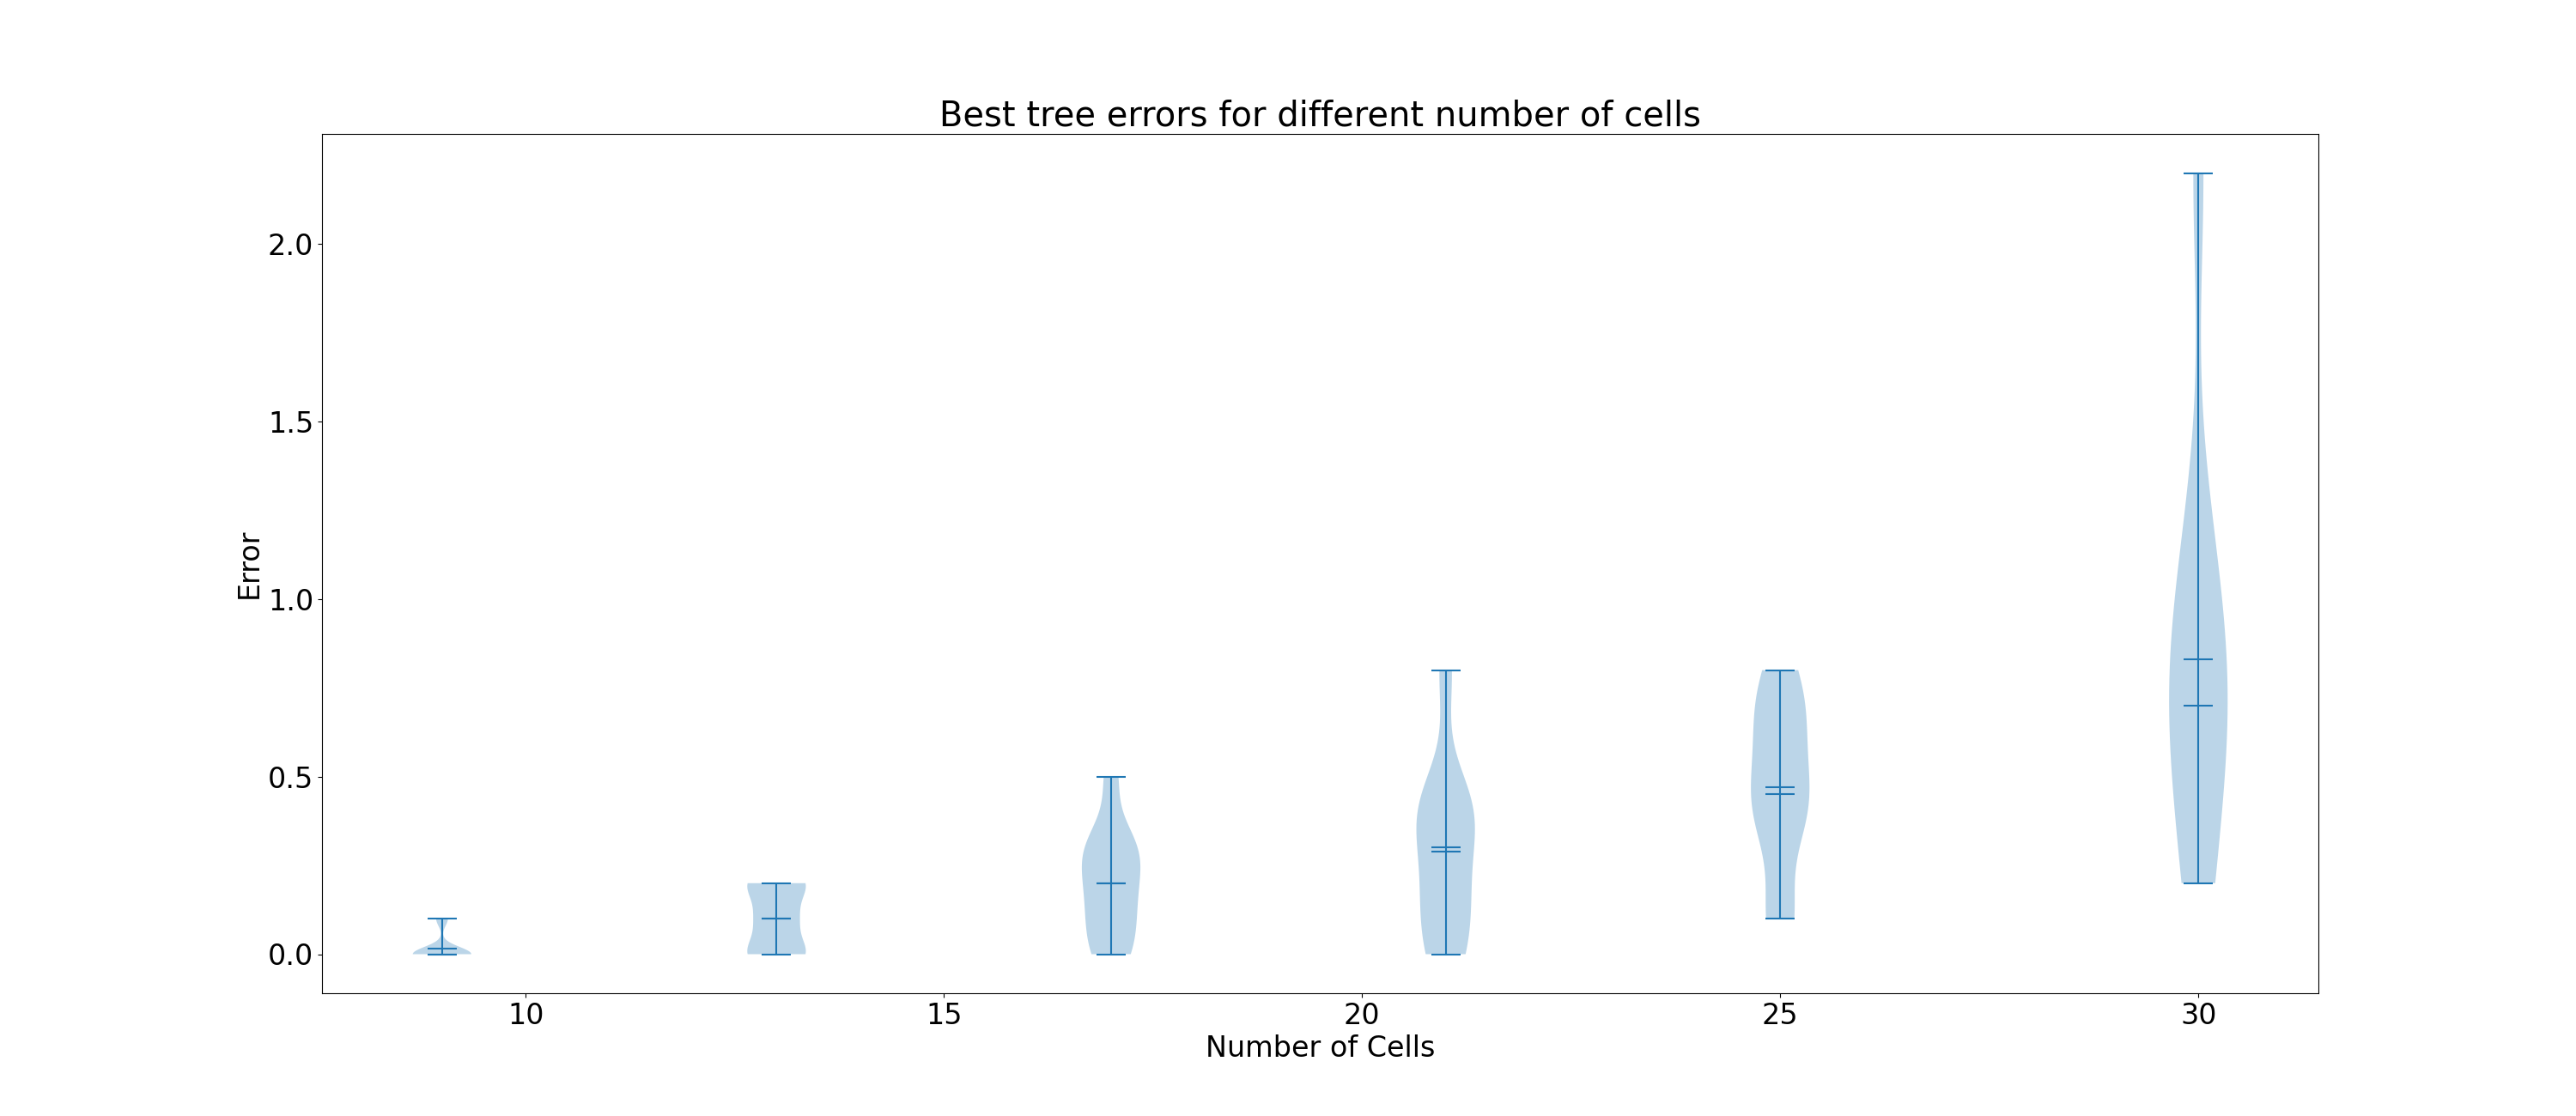
\includegraphics[width=\textwidth]{img/res/sy_N_Err}
	\caption{‌نتیجه اجرای روش پیشنهادی برای تعداد نمونه‌های مختلف}
	\label{fig:sy_n_err}
\end{figure}
حال برای اینکه متوجه شویم آیا این افزایش خطا بخاطر ضعف روش پیشنهادی است یا ماهیت داده‌های ورودی میزان خطا را در هر اجرا بر تعداد خانه‌های ماتریس $D$ تقسیم می‌کنیم که در آن صورت به نمودار شکل \ref{fig:sy_n_err_mean} می‌رسیم.
\begin{figure}[!ht]
	\centering
	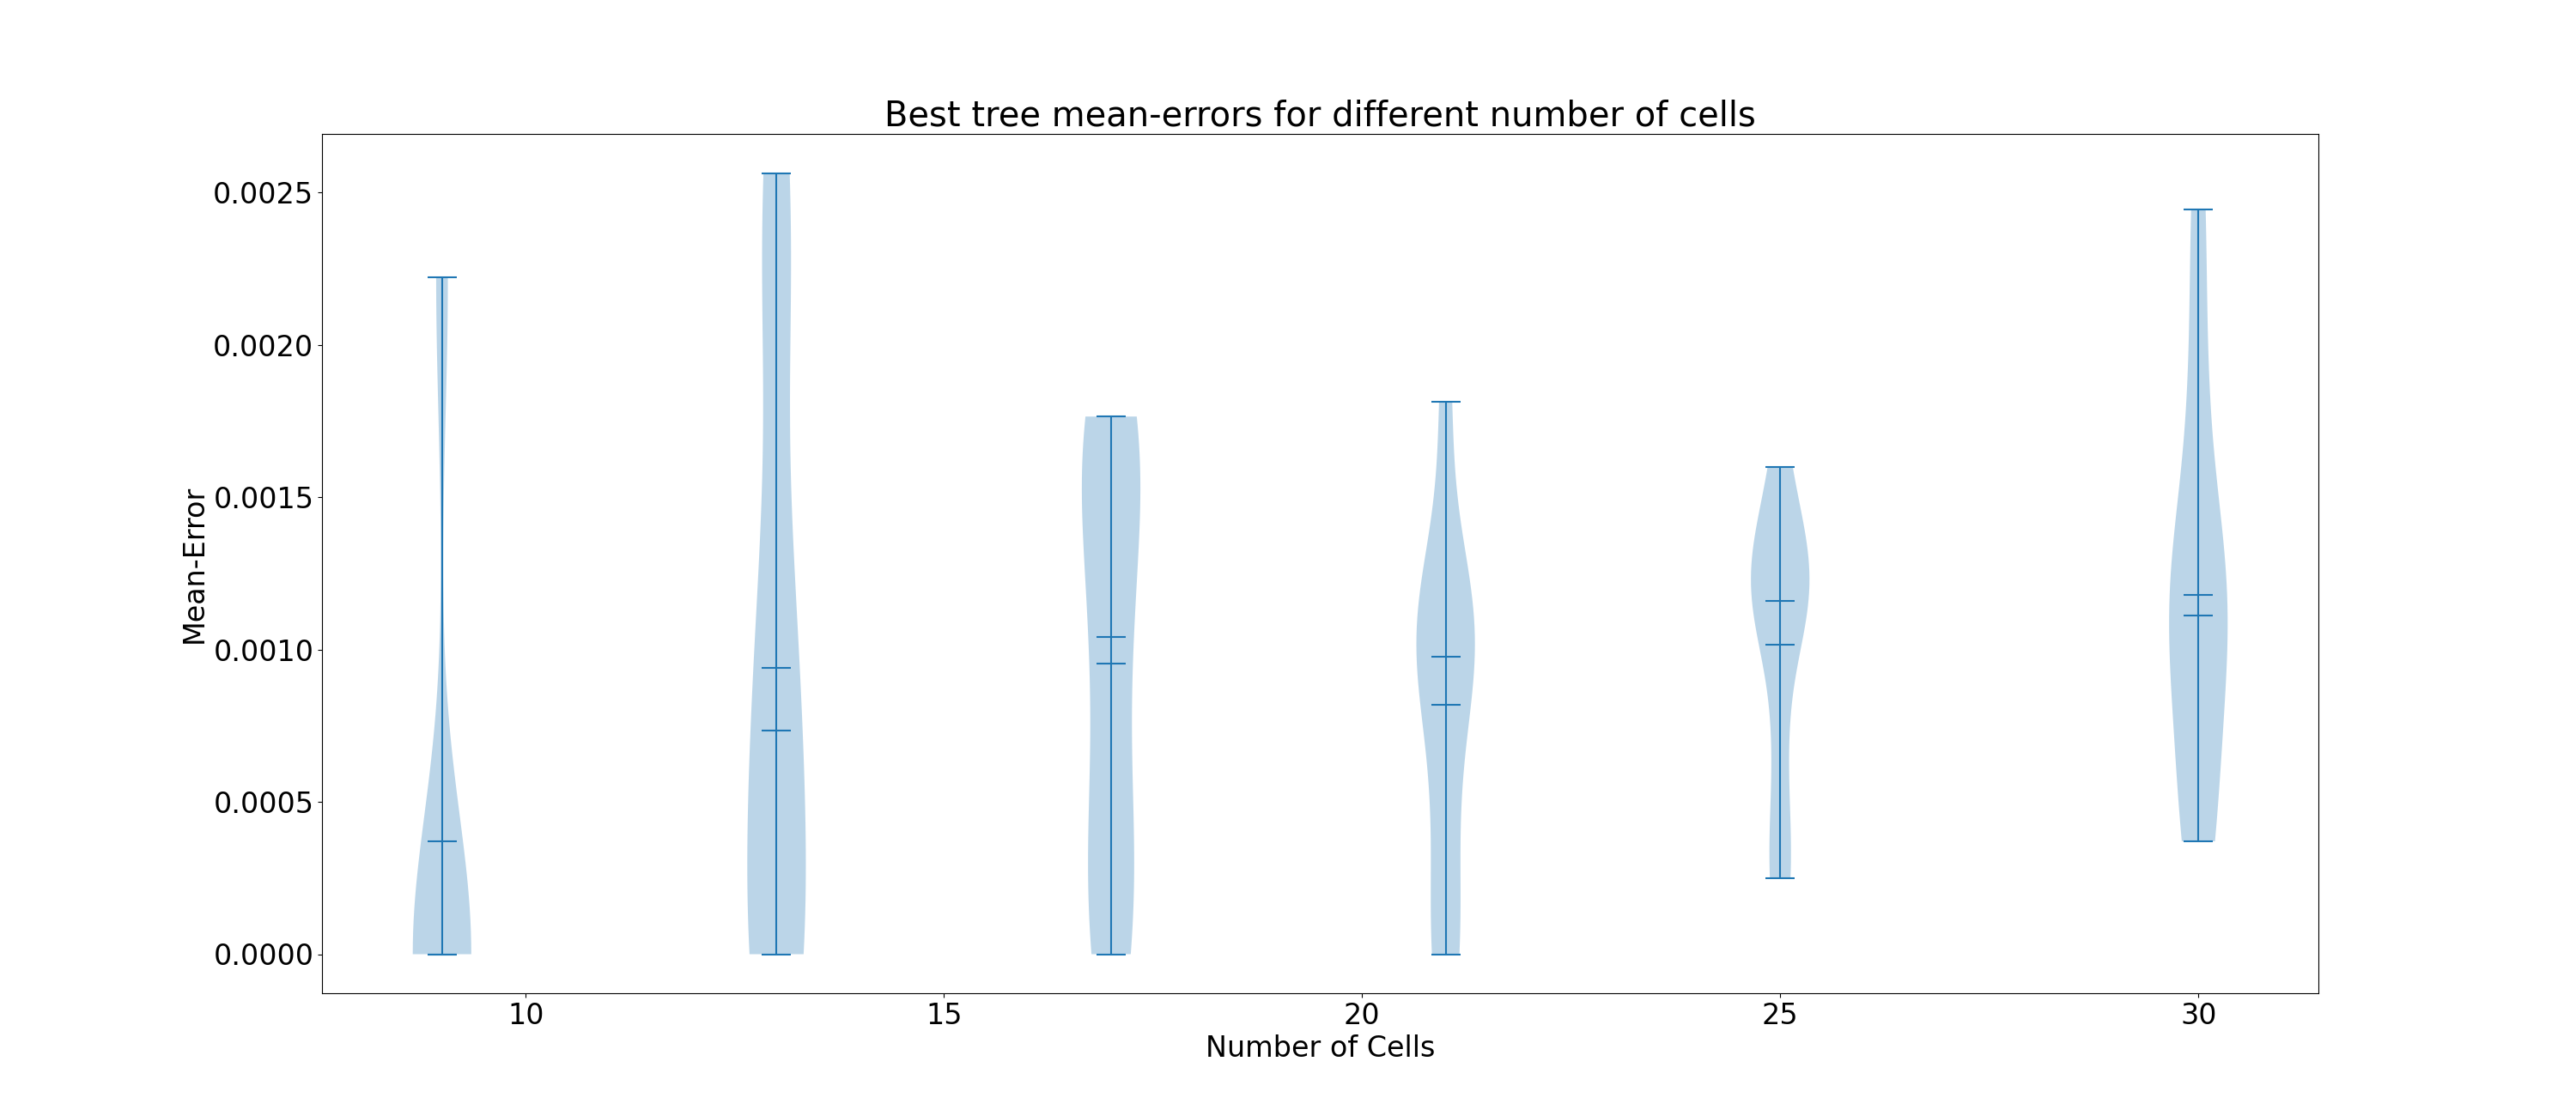
\includegraphics[width=\textwidth]{img/res/sy_N_Err_mean}
	\caption{‌نتیجه اجرای روش پیشنهادی برای تعداد نمونه‌های مختلف}
	\label{fig:sy_n_err_mean}
\end{figure}
در این نمودار جدید مشخص می‌شود که با افزایش اندازه ماتریس ورودی روش پیشنهادی سعی می‌کند تا خطا را به ازای هر داده کنترل کند که نشان از کارآمدی روش پیشنهادی می‌باشد.

\subsection{نتایج بر روی داده‌های حقیقی}
در این قسمت به ارائه گزارش و نتایج حاصل از روش‌های پیشنهادی با استفاده از داده‌های حقیقی برای بدست آوردن درخت فیلوژنی خواهیم پرداخت.
\subsubsection{نتایج بهینه‌سازی درخت ژنی}
همان‌طور که در فصل قبل بیان شد، یکی از روش‌های بدست آوردن درخت فیلوژنی استفاده از یک درخت تصادفی نابهینه ژنی بود که طی تکرار گام‌هایی سعی در تغییر اتصالات و یافتن درخت بهینه داشت که بتواند روند صحیح تغییرات ژنی را در تومور مورد نظر نمایش دهد.
نتیجه بدست آمده بر روی پایگاه داده حقیقی \lr{Navin} به شرح زیر می‌باشد که عکس \ref{fig:sn_initial_T} درخت تصادفی اولیه الگوریتم را نشان می‌دهد که انرژی آن نیز بالای تصویر نوشته شده است.\\
\begin{figure}[!ht]
	\centering
	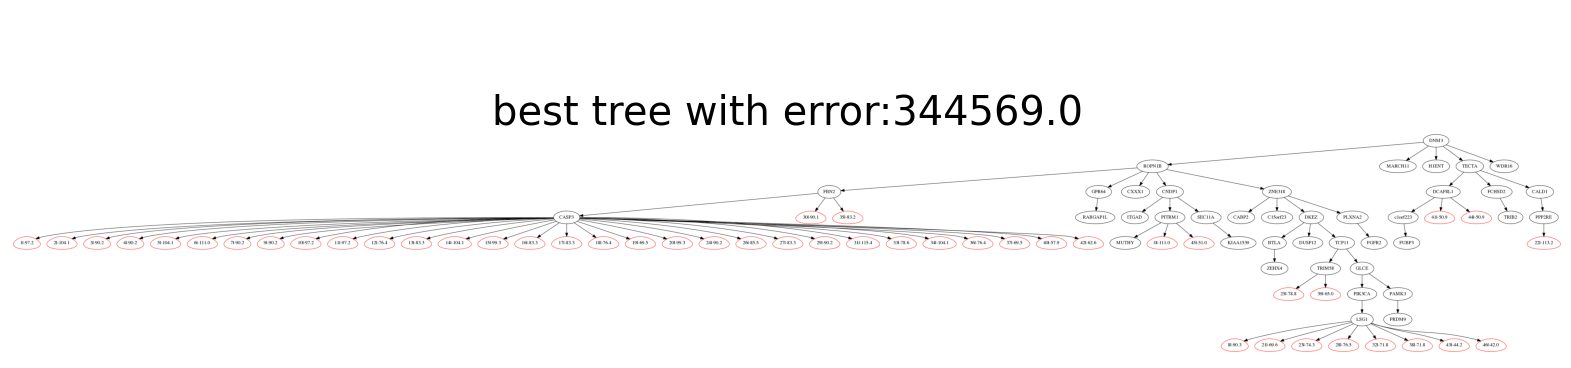
\includegraphics[width=\textwidth]{img/res/sn_initial_tree}
	\caption{درخت تصادفی اولیه}
	\label{fig:sn_initial_T}
\end{figure}

تصویر \ref{fig:Gene_ٍenergy_chart} نیز نمودار تغییر انرژی را طی گام‌های مختلف نمایش پیشنهادی مشخص می‌کند.
\begin{figure}[!ht]
	\centering
	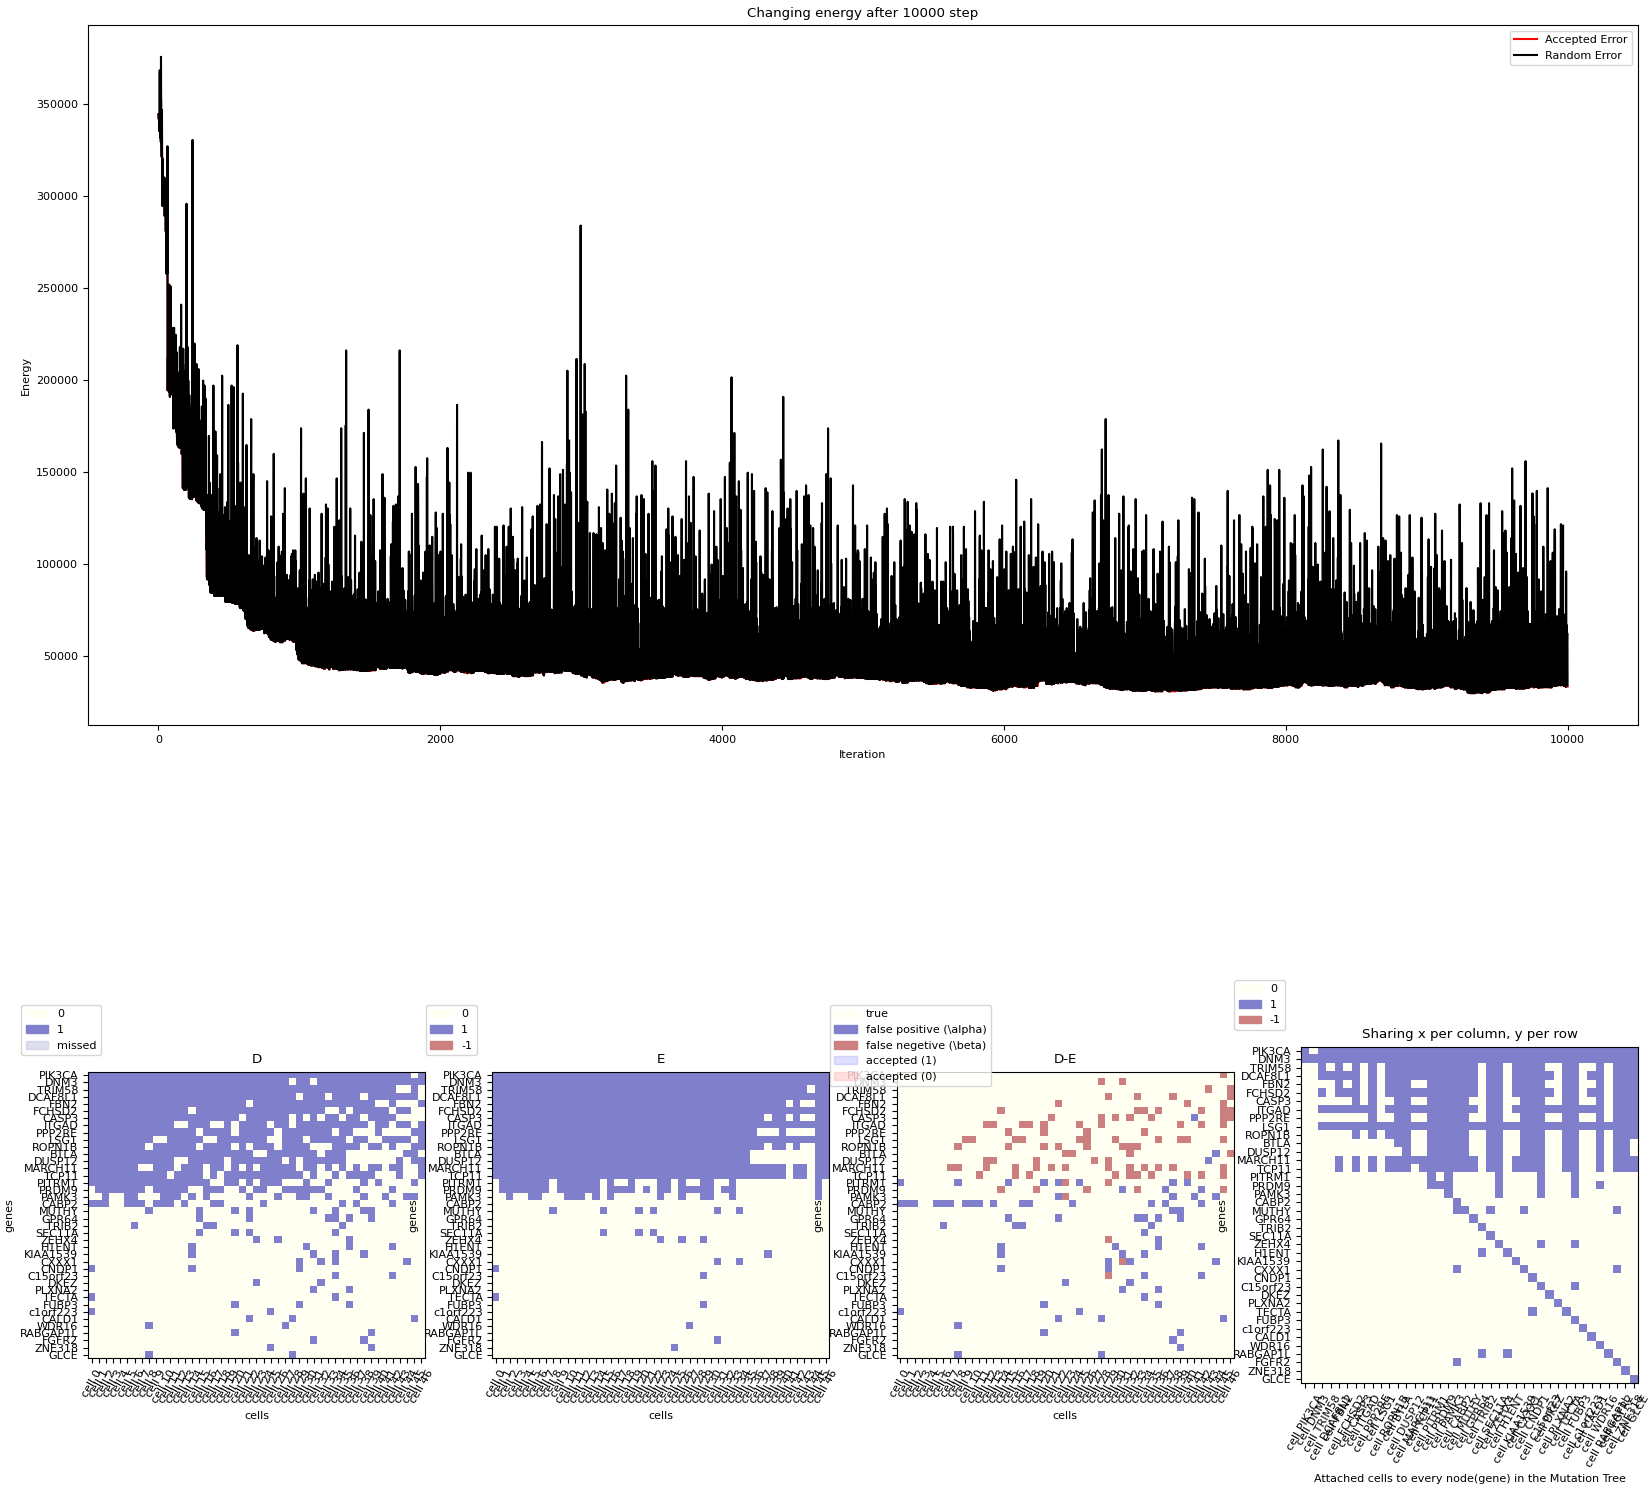
\includegraphics[width=\textwidth]{img/res/sn_benchmark}
	\caption{نمودار تغییر انرژی در طی گام‌های مختلف}
	\label{fig:Gene_ٍenergy_chart}
\end{figure}
در نهایت تصویر بهترین درخت یافته شده به همراه انرژی آن.
\begin{figure}[!ht]
	\centering
	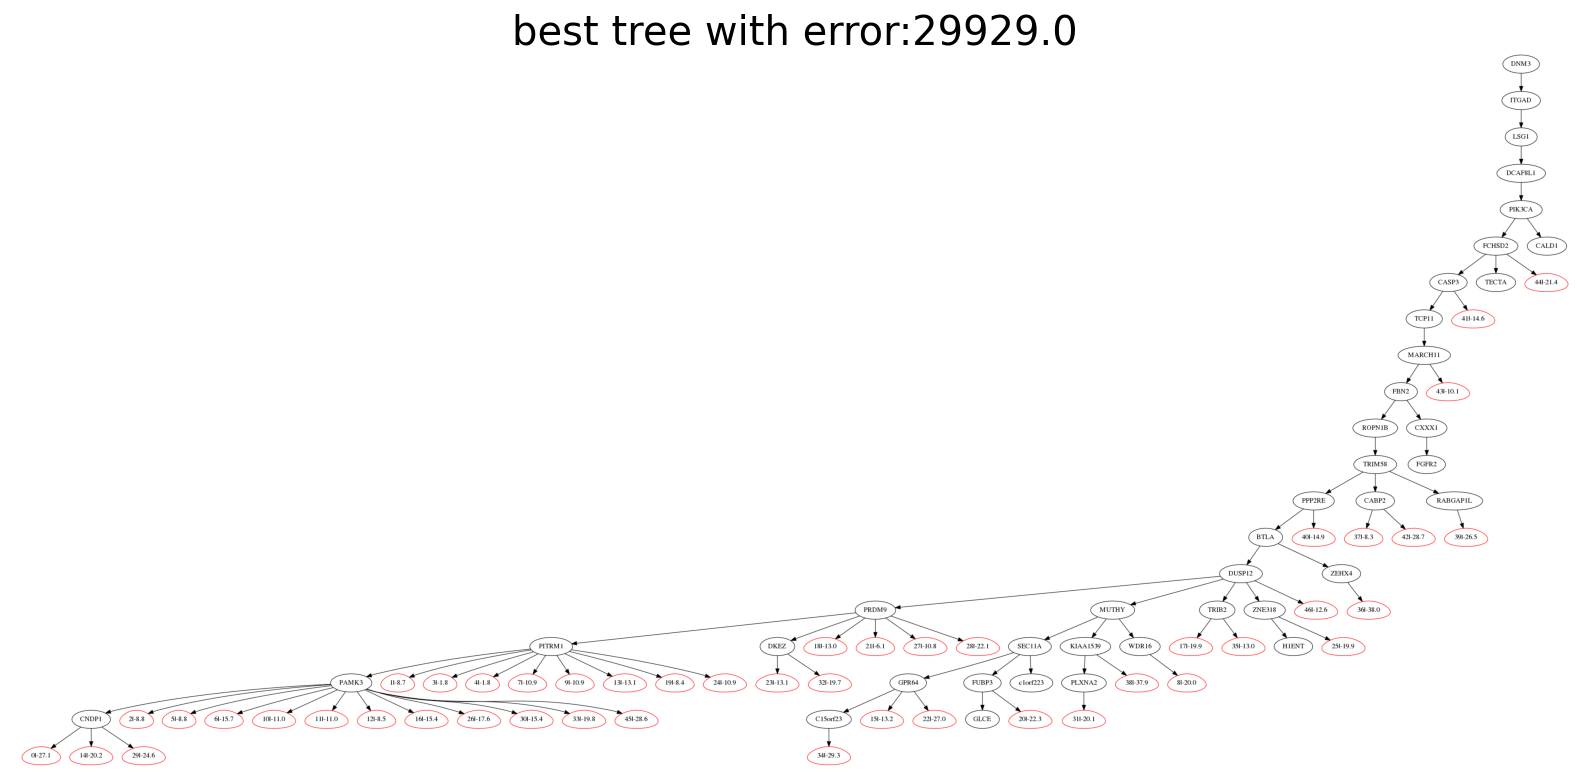
\includegraphics[width=\textwidth]{img/res/sn_best_tree}
	\caption{بهترین درخت یافته‌شده و خروجی الگوریتم برای مقاله \lr{SCITE}}
	\label{fig:Gene_ٍbest_tree}
\end{figure}

در نهایت برای مقایسه نیز تصویر درخت حاصله در مقاله اصلی \lr{SCITE} را در شکل \ref{fig:Gene_ٍSCITE} نمایش داده شده است.
\begin{figure}[!ht]
	\centering
	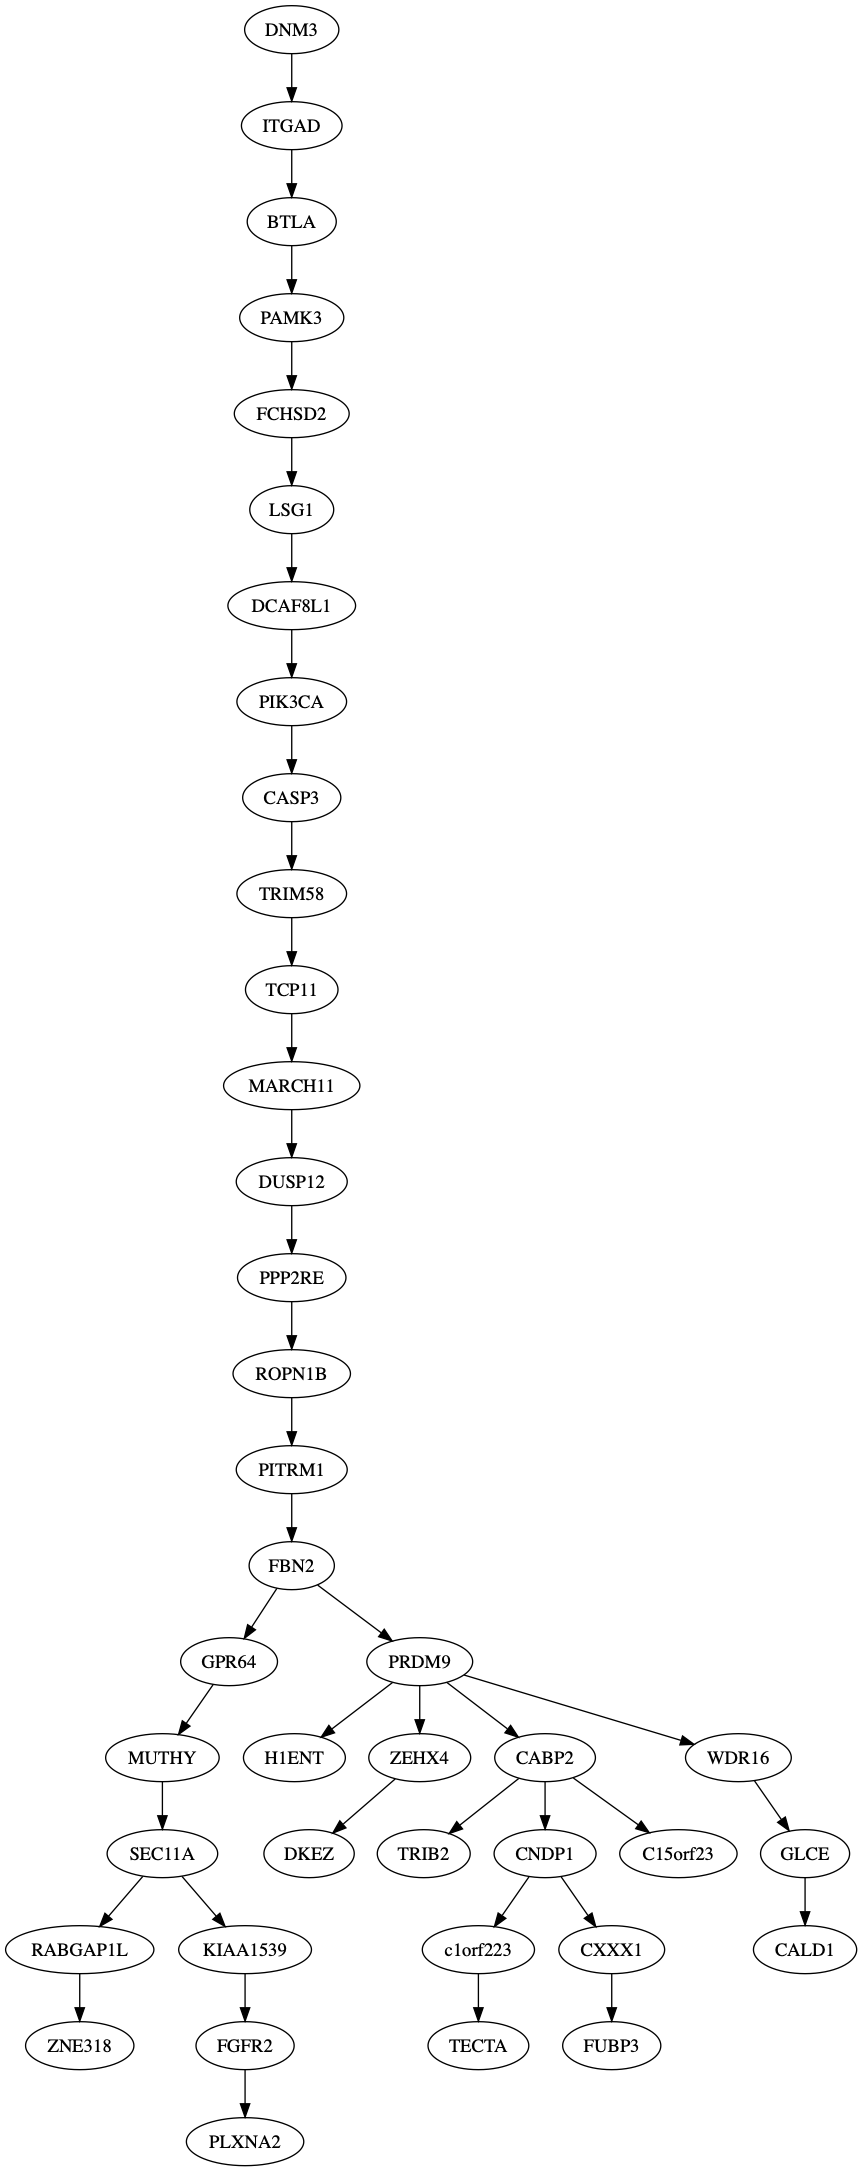
\includegraphics[width=0.6\textwidth]{img/res/SCITE}
	\caption{درخت بدست آمده در مقاله \lr{SCITE}}
	\label{fig:Gene_ٍSCITE}
\end{figure}
همان‌طور که مشخص است مقدار انرژی بدست آمده برای خروجی الگوریتم پیشنهادی بهتر (کمتر) از انرژی درخت \lr{SCITE} می‌باشد که دلیل بر بهینه‌تر بودن درخت روش پیشنهادی ارائه شده در این گزارش است.

\newpage
\section{گام‌های آتی}
در ادامه برای تکمیل روش پیشنهادی در دو قسمت نیاز به بهبود وجود دارد.\\
قسمت اول مربوط به درخت اولیه است و قسمت دیگر مربوط به سرعت \lr{MCMC} می‌باشد.
\subsection{بهبود در ساخت درخت اولیه}
در حال حاضر ما درخت اولیه را به صورت تصادفی انتخاب می‌کنیم که می‌توان در این مرحله درخت اولیه را با استفاده از مفروضات مدل مکان‌های بی‌نهایت و با توجه به ماتریس ورودی بهبود بخشید. این کار باعث می‌شود تا شروع الگوریتم از نقطه بهتری باشد که در این صورت هم گام‌های لازم برای رسیدن به درخت بهینه می‌تواند کمتر شود و هم اینکه احتمال قرار گرفتن در نقاط اکسترمم نسبی را کاهش می‌دهیم.

\subsection{افزایش سرعت همگرایی \lr{MCMC}}
در این بخش نیاز است تا در دو قسمت روش پیشنهادی بهبود یابد.
\subsubsection{تنوع در گام‌ها با استراتژی معقول}
برای این بخش کاری که باید انجام شود این است که بتوان برای افزایش سرعت همگرایی از روش‌های مختلف در گام‌ها استفاده کرد. برای مثال در حال حاضر می‌توان از سه روش مختلف در هر گام استفاده نمود. روش اول تعویض دو نود در درخت می‌باشد. روش دوم جدایی یک زیر درخت و اتصال آن به محلی دیگر می‌باشد و  در نهایت روش سوم تعویض دو زیر درخت با یکدیگر می‌باشد. با انتخاب یک استراتژی مناسب بین هرکدام از این روش‌ها در گام‌های مختلف احتمالا بتوان سرعت همگرایی را افزایش داد.

\subsubsection{قرار دادن احتمال وزن‌دار به ازای هر انتخاب}
در حال حاضر ما در هرکدام از روش‌های مختلف که در بخش قبل برای گام‌های \lr{MCMC} بیان کردیم، انتخاب نودها را به صورت کاملا یکنواخت انجام می‌دهیم. در صورتی که احتمالا بتوان با تعریف فرمولی مناسب این احتمال انتخاب بین نودهای مختلف در درخت را از حالت یکنواخت خارج کرد و در نتیجه مجددا سرعت همگرایی الگوریتم را افزایش داد.
